\documentclass[twoside]{book}

% Packages required by doxygen
\usepackage{fixltx2e}
\usepackage{calc}
\usepackage{doxygen}
\usepackage[export]{adjustbox} % also loads graphicx
\usepackage{graphicx}
\usepackage[utf8]{inputenc}
\usepackage{makeidx}
\usepackage{multicol}
\usepackage{multirow}
\PassOptionsToPackage{warn}{textcomp}
\usepackage{textcomp}
\usepackage[nointegrals]{wasysym}
\usepackage[table]{xcolor}

% NLS support packages
\usepackage{polski}
\usepackage[T1]{fontenc}

% Font selection
\usepackage[T1]{fontenc}
\usepackage[scaled=.90]{helvet}
\usepackage{courier}
\usepackage{amssymb}
\usepackage{sectsty}
\renewcommand{\familydefault}{\sfdefault}
\allsectionsfont{%
  \fontseries{bc}\selectfont%
  \color{darkgray}%
}
\renewcommand{\DoxyLabelFont}{%
  \fontseries{bc}\selectfont%
  \color{darkgray}%
}
\newcommand{\+}{\discretionary{\mbox{\scriptsize$\hookleftarrow$}}{}{}}

% Page & text layout
\usepackage{geometry}
\geometry{%
  a4paper,%
  top=2.5cm,%
  bottom=2.5cm,%
  left=2.5cm,%
  right=2.5cm%
}
\tolerance=750
\hfuzz=15pt
\hbadness=750
\setlength{\emergencystretch}{15pt}
\setlength{\parindent}{0cm}
\setlength{\parskip}{3ex plus 2ex minus 2ex}
\makeatletter
\renewcommand{\paragraph}{%
  \@startsection{paragraph}{4}{0ex}{-1.0ex}{1.0ex}{%
    \normalfont\normalsize\bfseries\SS@parafont%
  }%
}
\renewcommand{\subparagraph}{%
  \@startsection{subparagraph}{5}{0ex}{-1.0ex}{1.0ex}{%
    \normalfont\normalsize\bfseries\SS@subparafont%
  }%
}
\makeatother

% Headers & footers
\usepackage{fancyhdr}
\pagestyle{fancyplain}
\fancyhead[LE]{\fancyplain{}{\bfseries\thepage}}
\fancyhead[CE]{\fancyplain{}{}}
\fancyhead[RE]{\fancyplain{}{\bfseries\leftmark}}
\fancyhead[LO]{\fancyplain{}{\bfseries\rightmark}}
\fancyhead[CO]{\fancyplain{}{}}
\fancyhead[RO]{\fancyplain{}{\bfseries\thepage}}
\fancyfoot[LE]{\fancyplain{}{}}
\fancyfoot[CE]{\fancyplain{}{}}
\fancyfoot[RE]{\fancyplain{}{\bfseries\scriptsize Wygenerowano przez Doxygen }}
\fancyfoot[LO]{\fancyplain{}{\bfseries\scriptsize Wygenerowano przez Doxygen }}
\fancyfoot[CO]{\fancyplain{}{}}
\fancyfoot[RO]{\fancyplain{}{}}
\renewcommand{\footrulewidth}{0.4pt}
\renewcommand{\chaptermark}[1]{%
  \markboth{#1}{}%
}
\renewcommand{\sectionmark}[1]{%
  \markright{\thesection\ #1}%
}

% Indices & bibliography
\usepackage{natbib}
\usepackage[titles]{tocloft}
\setcounter{tocdepth}{3}
\setcounter{secnumdepth}{5}
\makeindex

% Hyperlinks (required, but should be loaded last)
\usepackage{ifpdf}
\ifpdf
  \usepackage[pdftex,pagebackref=true]{hyperref}
\else
  \usepackage[ps2pdf,pagebackref=true]{hyperref}
\fi
\hypersetup{%
  colorlinks=true,%
  linkcolor=blue,%
  citecolor=blue,%
  unicode%
}

% Custom commands
\newcommand{\clearemptydoublepage}{%
  \newpage{\pagestyle{empty}\cleardoublepage}%
}

\usepackage{caption}
\captionsetup{labelsep=space,justification=centering,font={bf},singlelinecheck=off,skip=4pt,position=top}

%===== C O N T E N T S =====

\begin{document}

% Titlepage & ToC
\hypersetup{pageanchor=false,
             bookmarksnumbered=true,
             pdfencoding=unicode
            }
\pagenumbering{roman}
\begin{titlepage}
\vspace*{7cm}
\begin{center}%
{\Large Window \\[1ex]\large 1 }\\
\vspace*{1cm}
{\large Wygenerowano przez Doxygen 1.8.11}\\
\end{center}
\end{titlepage}
\clearemptydoublepage
\tableofcontents
\clearemptydoublepage
\pagenumbering{arabic}
\hypersetup{pageanchor=true}

%--- Begin generated contents ---
\chapter{Indeks hierarchiczny}
\section{Hierarchia klas}
Ta lista dziedziczenia posortowana jest z grubsza, choć nie całkowicie, alfabetycznie\+:\begin{DoxyCompactList}
\item \contentsline{section}{Component}{\pageref{classComponent}}{}
\begin{DoxyCompactList}
\item \contentsline{section}{Checkbox}{\pageref{classCheckbox}}{}
\item \contentsline{section}{Text}{\pageref{classText}}{}
\begin{DoxyCompactList}
\item \contentsline{section}{Button}{\pageref{classButton}}{}
\item \contentsline{section}{Input\+\_\+table}{\pageref{classInput__table}}{}
\item \contentsline{section}{List}{\pageref{classList}}{}
\end{DoxyCompactList}
\end{DoxyCompactList}
\end{DoxyCompactList}

\chapter{Indeks klas}
\section{Lista klas}
Tutaj znajdują się klasy, struktury, unie i interfejsy wraz z ich krótkimi opisami\+:\begin{DoxyCompactList}
\item\contentsline{section}{\hyperlink{classButton}{Button} }{\pageref{classButton}}{}
\item\contentsline{section}{\hyperlink{classCheckbox}{Checkbox} }{\pageref{classCheckbox}}{}
\item\contentsline{section}{\hyperlink{classComponent}{Component} }{\pageref{classComponent}}{}
\item\contentsline{section}{\hyperlink{classInput__table}{Input\+\_\+table} }{\pageref{classInput__table}}{}
\item\contentsline{section}{\hyperlink{classText}{Text} }{\pageref{classText}}{}
\end{DoxyCompactList}

\chapter{Indeks plików}
\section{Lista plików}
Tutaj znajduje się lista wszystkich plików z ich krótkimi opisami\+:\begin{DoxyCompactList}
\item\contentsline{section}{\hyperlink{main_8cpp}{main.\+cpp} }{\pageref{main_8cpp}}{}
\item\contentsline{section}{\hyperlink{operating__sys_8cpp}{operating\+\_\+sys.\+cpp} }{\pageref{operating__sys_8cpp}}{}
\item\contentsline{section}{\hyperlink{operating__sys_8h}{operating\+\_\+sys.\+h} }{\pageref{operating__sys_8h}}{}
\item\contentsline{section}{\hyperlink{window_8cpp}{window.\+cpp} }{\pageref{window_8cpp}}{}
\item\contentsline{section}{\hyperlink{window_8h}{window.\+h} }{\pageref{window_8h}}{}
\end{DoxyCompactList}

\chapter{Dokumentacja klas}
\hypertarget{classButton}{}\section{Dokumentacja klasy Button}
\label{classButton}\index{Button@{Button}}


{\ttfamily \#include $<$window.\+h$>$}



Diagram dziedziczenia dla Button\nopagebreak
\begin{figure}[H]
\begin{center}
\leavevmode
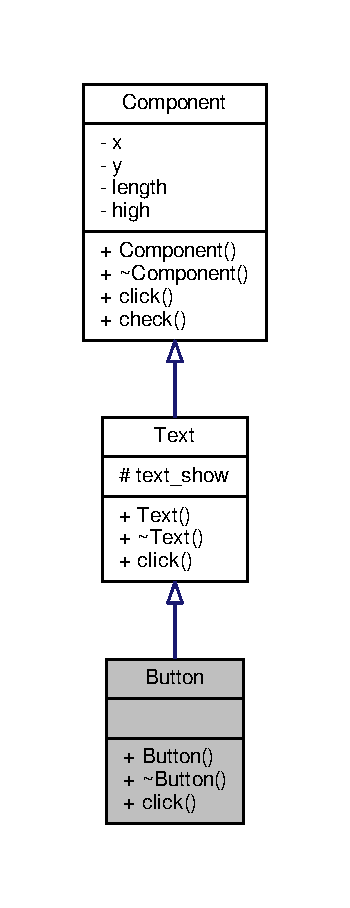
\includegraphics[width=168pt]{classButton__inherit__graph}
\end{center}
\end{figure}


Diagram współpracy dla Button\+:\nopagebreak
\begin{figure}[H]
\begin{center}
\leavevmode
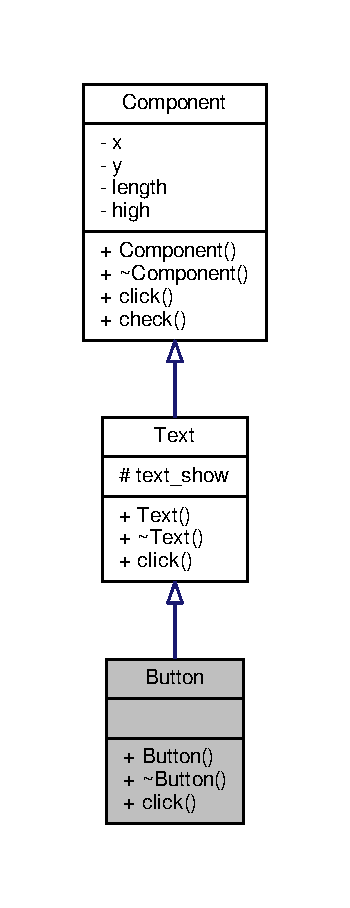
\includegraphics[width=168pt]{classButton__coll__graph}
\end{center}
\end{figure}
\subsection*{Metody publiczne}
\begin{DoxyCompactItemize}
\item 
\hyperlink{classButton_affc1899d8e846ffda38377637d675d29}{Button} (int x\+\_\+axe=0, int y\+\_\+axe=0, int length\+\_\+p=20, int high\+\_\+p=15, string tekst\+\_\+p=\char`\"{}Click \hyperlink{classButton}{Button}\char`\"{})
\item 
\hyperlink{classButton_a2a001eb9c3cc8ae54768a850dd345002}{$\sim$\+Button} ()
\item 
virtual void \hyperlink{classButton_a2fc33ec22217562b28ac6f02bda26c6e}{click} ()
\end{DoxyCompactItemize}


\subsection{Dokumentacja konstruktora i destruktora}
\index{Button@{Button}!Button@{Button}}
\index{Button@{Button}!Button@{Button}}
\subsubsection[{\texorpdfstring{Button(int x\+\_\+axe=0, int y\+\_\+axe=0, int length\+\_\+p=20, int high\+\_\+p=15, string tekst\+\_\+p=""Click Button"")}{Button(int x_axe=0, int y_axe=0, int length_p=20, int high_p=15, string tekst_p="Click Button")}}]{\setlength{\rightskip}{0pt plus 5cm}Button\+::\+Button (
\begin{DoxyParamCaption}
\item[{int}]{x\+\_\+axe = {\ttfamily 0}, }
\item[{int}]{y\+\_\+axe = {\ttfamily 0}, }
\item[{int}]{length\+\_\+p = {\ttfamily 20}, }
\item[{int}]{high\+\_\+p = {\ttfamily 15}, }
\item[{string}]{tekst\+\_\+p = {\ttfamily \char`\"{}Click~{\bf Button}\char`\"{}}}
\end{DoxyParamCaption}
)\hspace{0.3cm}{\ttfamily [inline]}}\hypertarget{classButton_affc1899d8e846ffda38377637d675d29}{}\label{classButton_affc1899d8e846ffda38377637d675d29}
\index{Button@{Button}!````~Button@{$\sim$\+Button}}
\index{````~Button@{$\sim$\+Button}!Button@{Button}}
\subsubsection[{\texorpdfstring{$\sim$\+Button()}{~Button()}}]{\setlength{\rightskip}{0pt plus 5cm}Button\+::$\sim$\+Button (
\begin{DoxyParamCaption}
{}
\end{DoxyParamCaption}
)\hspace{0.3cm}{\ttfamily [inline]}}\hypertarget{classButton_a2a001eb9c3cc8ae54768a850dd345002}{}\label{classButton_a2a001eb9c3cc8ae54768a850dd345002}


\subsection{Dokumentacja funkcji składowych}
\index{Button@{Button}!click@{click}}
\index{click@{click}!Button@{Button}}
\subsubsection[{\texorpdfstring{click()}{click()}}]{\setlength{\rightskip}{0pt plus 5cm}void Button\+::click (
\begin{DoxyParamCaption}
{}
\end{DoxyParamCaption}
)\hspace{0.3cm}{\ttfamily [virtual]}}\hypertarget{classButton_a2fc33ec22217562b28ac6f02bda26c6e}{}\label{classButton_a2fc33ec22217562b28ac6f02bda26c6e}


Reimplementowana z \hyperlink{classText_ab334ff82f41302f83bebf3eaf2516a84}{Text}.



Dokumentacja dla tej klasy została wygenerowana z plików\+:\begin{DoxyCompactItemize}
\item 
\hyperlink{window_8h}{window.\+h}\item 
\hyperlink{window_8cpp}{window.\+cpp}\end{DoxyCompactItemize}

\hypertarget{classCheckbox}{}\section{Dokumentacja klasy Checkbox}
\label{classCheckbox}\index{Checkbox@{Checkbox}}


{\ttfamily \#include $<$window.\+h$>$}



Diagram dziedziczenia dla Checkbox
\nopagebreak
\begin{figure}[H]
\begin{center}
\leavevmode
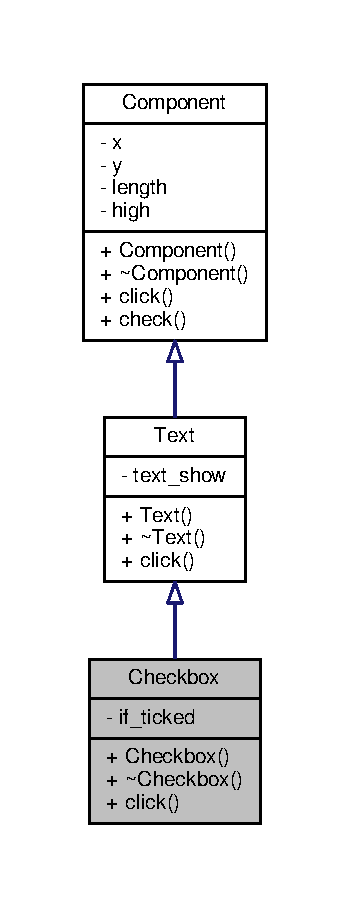
\includegraphics[height=550pt]{classCheckbox__inherit__graph}
\end{center}
\end{figure}


Diagram współpracy dla Checkbox\+:
\nopagebreak
\begin{figure}[H]
\begin{center}
\leavevmode
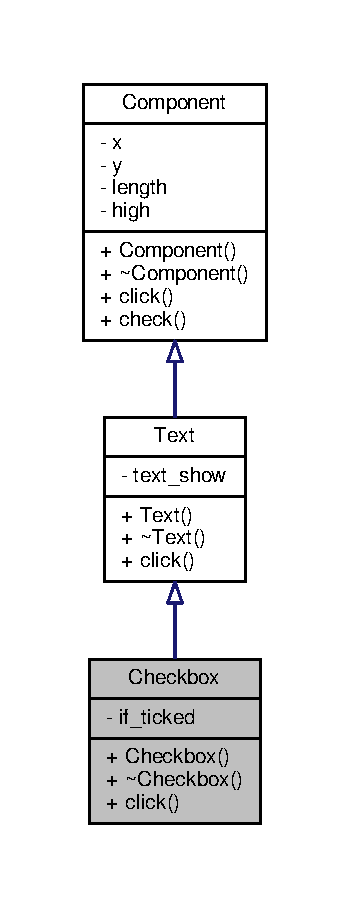
\includegraphics[height=550pt]{classCheckbox__coll__graph}
\end{center}
\end{figure}
\subsection*{Metody publiczne}
\begin{DoxyCompactItemize}
\item 
\hyperlink{classCheckbox_a44d2ffeb1990a715b7d99f7ad48d36cf}{Checkbox} (int x\+\_\+axe=0, int y\+\_\+axe=0, int length\+\_\+p=8, int high\+\_\+p=8, string tekst\+\_\+p=\char`\"{}Tick \hyperlink{classCheckbox}{Checkbox}\char`\"{}, bool if\+\_\+ticked\+\_\+par=false)
\item 
\hyperlink{classCheckbox_a828c1436e32c8be0d9d395286d8e6bfe}{$\sim$\+Checkbox} ()
\item 
virtual void \hyperlink{classCheckbox_afd75946a43da1dcba8e6f04f00df34ee}{click} ()
\end{DoxyCompactItemize}
\subsection*{Atrybuty prywatne}
\begin{DoxyCompactItemize}
\item 
bool \hyperlink{classCheckbox_a3a35b7a1272d8aa2d349d0e8820220b5}{if\+\_\+ticked}
\end{DoxyCompactItemize}


\subsection{Dokumentacja konstruktora i destruktora}
\index{Checkbox@{Checkbox}!Checkbox@{Checkbox}}
\index{Checkbox@{Checkbox}!Checkbox@{Checkbox}}
\subsubsection[{\texorpdfstring{Checkbox(int x\+\_\+axe=0, int y\+\_\+axe=0, int length\+\_\+p=8, int high\+\_\+p=8, string tekst\+\_\+p=""Tick Checkbox"", bool if\+\_\+ticked\+\_\+par=false)}{Checkbox(int x_axe=0, int y_axe=0, int length_p=8, int high_p=8, string tekst_p="Tick Checkbox", bool if_ticked_par=false)}}]{\setlength{\rightskip}{0pt plus 5cm}Checkbox\+::\+Checkbox (
\begin{DoxyParamCaption}
\item[{int}]{x\+\_\+axe = {\ttfamily 0}, }
\item[{int}]{y\+\_\+axe = {\ttfamily 0}, }
\item[{int}]{length\+\_\+p = {\ttfamily 8}, }
\item[{int}]{high\+\_\+p = {\ttfamily 8}, }
\item[{string}]{tekst\+\_\+p = {\ttfamily \char`\"{}Tick~{\bf Checkbox}\char`\"{}}, }
\item[{bool}]{if\+\_\+ticked\+\_\+par = {\ttfamily false}}
\end{DoxyParamCaption}
)\hspace{0.3cm}{\ttfamily [inline]}}\hypertarget{classCheckbox_a44d2ffeb1990a715b7d99f7ad48d36cf}{}\label{classCheckbox_a44d2ffeb1990a715b7d99f7ad48d36cf}
\index{Checkbox@{Checkbox}!````~Checkbox@{$\sim$\+Checkbox}}
\index{````~Checkbox@{$\sim$\+Checkbox}!Checkbox@{Checkbox}}
\subsubsection[{\texorpdfstring{$\sim$\+Checkbox()}{~Checkbox()}}]{\setlength{\rightskip}{0pt plus 5cm}Checkbox\+::$\sim$\+Checkbox (
\begin{DoxyParamCaption}
{}
\end{DoxyParamCaption}
)\hspace{0.3cm}{\ttfamily [inline]}}\hypertarget{classCheckbox_a828c1436e32c8be0d9d395286d8e6bfe}{}\label{classCheckbox_a828c1436e32c8be0d9d395286d8e6bfe}


\subsection{Dokumentacja funkcji składowych}
\index{Checkbox@{Checkbox}!click@{click}}
\index{click@{click}!Checkbox@{Checkbox}}
\subsubsection[{\texorpdfstring{click()}{click()}}]{\setlength{\rightskip}{0pt plus 5cm}void Checkbox\+::click (
\begin{DoxyParamCaption}
{}
\end{DoxyParamCaption}
)\hspace{0.3cm}{\ttfamily [virtual]}}\hypertarget{classCheckbox_afd75946a43da1dcba8e6f04f00df34ee}{}\label{classCheckbox_afd75946a43da1dcba8e6f04f00df34ee}


Reimplementowana z \hyperlink{classButton_a2fc33ec22217562b28ac6f02bda26c6e}{Button}.



\subsection{Dokumentacja atrybutów składowych}
\index{Checkbox@{Checkbox}!if\+\_\+ticked@{if\+\_\+ticked}}
\index{if\+\_\+ticked@{if\+\_\+ticked}!Checkbox@{Checkbox}}
\subsubsection[{\texorpdfstring{if\+\_\+ticked}{if_ticked}}]{\setlength{\rightskip}{0pt plus 5cm}bool Checkbox\+::if\+\_\+ticked\hspace{0.3cm}{\ttfamily [private]}}\hypertarget{classCheckbox_a3a35b7a1272d8aa2d349d0e8820220b5}{}\label{classCheckbox_a3a35b7a1272d8aa2d349d0e8820220b5}


Dokumentacja dla tej klasy została wygenerowana z plików\+:\begin{DoxyCompactItemize}
\item 
\hyperlink{window_8h}{window.\+h}\item 
\hyperlink{window_8cpp}{window.\+cpp}\end{DoxyCompactItemize}

\hypertarget{classComponent}{}\section{Dokumentacja klasy Component}
\label{classComponent}\index{Component@{Component}}


{\ttfamily \#include $<$window.\+h$>$}



Diagram dziedziczenia dla Component
\nopagebreak
\begin{figure}[H]
\begin{center}
\leavevmode
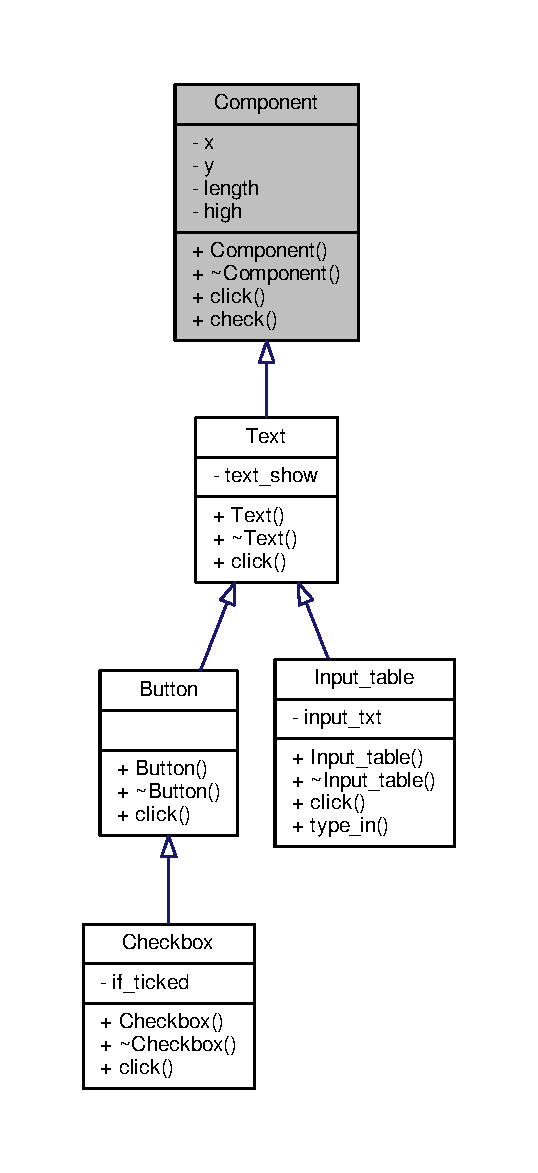
\includegraphics[width=348pt]{classComponent__inherit__graph}
\end{center}
\end{figure}


Diagram współpracy dla Component\+:
\nopagebreak
\begin{figure}[H]
\begin{center}
\leavevmode
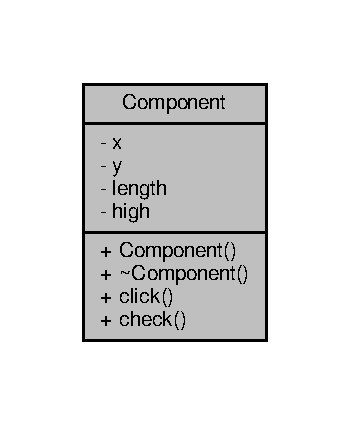
\includegraphics[width=168pt]{classComponent__coll__graph}
\end{center}
\end{figure}
\subsection*{Metody publiczne}
\begin{DoxyCompactItemize}
\item 
\hyperlink{classComponent_a24ce4a41eb6f0c89a8d874e19dcc46eb}{Component} (int x\+\_\+axe=0, int y\+\_\+axe=0, int length\+\_\+p=50, int high\+\_\+p=30)
\item 
virtual \hyperlink{classComponent_a2e9aa4348314d981f05f67397ad2f872}{$\sim$\+Component} ()
\item 
virtual void \hyperlink{classComponent_a247f6f0204b68a7efb9059cf709fe6ea}{click} ()=0
\item 
int \hyperlink{classComponent_abbe0759c6c9476750a086fe620d322d7}{check} (int x\+\_\+axe, int y\+\_\+axe)
\end{DoxyCompactItemize}
\subsection*{Atrybuty chronione}
\begin{DoxyCompactItemize}
\item 
int \hyperlink{classComponent_a3fe84cea3e41ac363349595e1a92a5b6}{x}
\item 
int \hyperlink{classComponent_a3cbb2a0f076a05810ad64ac22ea10402}{y}
\item 
int \hyperlink{classComponent_a4d25a50d4bfa8fde7f75478eadcd5661}{length}
\item 
int \hyperlink{classComponent_aff8a286217041306964f2207b86522b3}{high}
\end{DoxyCompactItemize}


\subsection{Dokumentacja konstruktora i destruktora}
\index{Component@{Component}!Component@{Component}}
\index{Component@{Component}!Component@{Component}}
\subsubsection[{\texorpdfstring{Component(int x\+\_\+axe=0, int y\+\_\+axe=0, int length\+\_\+p=50, int high\+\_\+p=30)}{Component(int x_axe=0, int y_axe=0, int length_p=50, int high_p=30)}}]{\setlength{\rightskip}{0pt plus 5cm}Component\+::\+Component (
\begin{DoxyParamCaption}
\item[{int}]{x\+\_\+axe = {\ttfamily 0}, }
\item[{int}]{y\+\_\+axe = {\ttfamily 0}, }
\item[{int}]{length\+\_\+p = {\ttfamily 50}, }
\item[{int}]{high\+\_\+p = {\ttfamily 30}}
\end{DoxyParamCaption}
)\hspace{0.3cm}{\ttfamily [inline]}}\hypertarget{classComponent_a24ce4a41eb6f0c89a8d874e19dcc46eb}{}\label{classComponent_a24ce4a41eb6f0c89a8d874e19dcc46eb}
\index{Component@{Component}!````~Component@{$\sim$\+Component}}
\index{````~Component@{$\sim$\+Component}!Component@{Component}}
\subsubsection[{\texorpdfstring{$\sim$\+Component()}{~Component()}}]{\setlength{\rightskip}{0pt plus 5cm}virtual Component\+::$\sim$\+Component (
\begin{DoxyParamCaption}
{}
\end{DoxyParamCaption}
)\hspace{0.3cm}{\ttfamily [inline]}, {\ttfamily [virtual]}}\hypertarget{classComponent_a2e9aa4348314d981f05f67397ad2f872}{}\label{classComponent_a2e9aa4348314d981f05f67397ad2f872}


\subsection{Dokumentacja funkcji składowych}
\index{Component@{Component}!check@{check}}
\index{check@{check}!Component@{Component}}
\subsubsection[{\texorpdfstring{check(int x\+\_\+axe, int y\+\_\+axe)}{check(int x_axe, int y_axe)}}]{\setlength{\rightskip}{0pt plus 5cm}int Component\+::check (
\begin{DoxyParamCaption}
\item[{int}]{x\+\_\+axe, }
\item[{int}]{y\+\_\+axe}
\end{DoxyParamCaption}
)}\hypertarget{classComponent_abbe0759c6c9476750a086fe620d322d7}{}\label{classComponent_abbe0759c6c9476750a086fe620d322d7}
\index{Component@{Component}!click@{click}}
\index{click@{click}!Component@{Component}}
\subsubsection[{\texorpdfstring{click()=0}{click()=0}}]{\setlength{\rightskip}{0pt plus 5cm}virtual void Component\+::click (
\begin{DoxyParamCaption}
{}
\end{DoxyParamCaption}
)\hspace{0.3cm}{\ttfamily [pure virtual]}}\hypertarget{classComponent_a247f6f0204b68a7efb9059cf709fe6ea}{}\label{classComponent_a247f6f0204b68a7efb9059cf709fe6ea}


Implementowany w \hyperlink{classList_a72af1f829c9b4ca5ee3cb3eaae52cf9a}{List}, \hyperlink{classInput__table_ac48806d103ed557c4b9a4eac4a021cf3}{Input\+\_\+table}, \hyperlink{classCheckbox_afd75946a43da1dcba8e6f04f00df34ee}{Checkbox}, \hyperlink{classButton_a2fc33ec22217562b28ac6f02bda26c6e}{Button} i \hyperlink{classText_ab334ff82f41302f83bebf3eaf2516a84}{Text}.



Oto graf wywoływań tej funkcji\+:\nopagebreak
\begin{figure}[H]
\begin{center}
\leavevmode
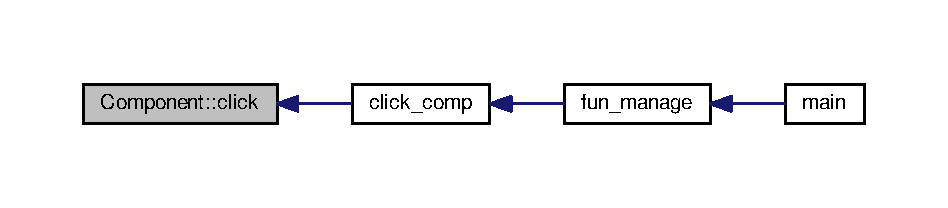
\includegraphics[width=350pt]{classComponent_a247f6f0204b68a7efb9059cf709fe6ea_icgraph}
\end{center}
\end{figure}




\subsection{Dokumentacja atrybutów składowych}
\index{Component@{Component}!high@{high}}
\index{high@{high}!Component@{Component}}
\subsubsection[{\texorpdfstring{high}{high}}]{\setlength{\rightskip}{0pt plus 5cm}int Component\+::high\hspace{0.3cm}{\ttfamily [protected]}}\hypertarget{classComponent_aff8a286217041306964f2207b86522b3}{}\label{classComponent_aff8a286217041306964f2207b86522b3}
\index{Component@{Component}!length@{length}}
\index{length@{length}!Component@{Component}}
\subsubsection[{\texorpdfstring{length}{length}}]{\setlength{\rightskip}{0pt plus 5cm}int Component\+::length\hspace{0.3cm}{\ttfamily [protected]}}\hypertarget{classComponent_a4d25a50d4bfa8fde7f75478eadcd5661}{}\label{classComponent_a4d25a50d4bfa8fde7f75478eadcd5661}
\index{Component@{Component}!x@{x}}
\index{x@{x}!Component@{Component}}
\subsubsection[{\texorpdfstring{x}{x}}]{\setlength{\rightskip}{0pt plus 5cm}int Component\+::x\hspace{0.3cm}{\ttfamily [protected]}}\hypertarget{classComponent_a3fe84cea3e41ac363349595e1a92a5b6}{}\label{classComponent_a3fe84cea3e41ac363349595e1a92a5b6}
\index{Component@{Component}!y@{y}}
\index{y@{y}!Component@{Component}}
\subsubsection[{\texorpdfstring{y}{y}}]{\setlength{\rightskip}{0pt plus 5cm}int Component\+::y\hspace{0.3cm}{\ttfamily [protected]}}\hypertarget{classComponent_a3cbb2a0f076a05810ad64ac22ea10402}{}\label{classComponent_a3cbb2a0f076a05810ad64ac22ea10402}


Dokumentacja dla tej klasy została wygenerowana z plików\+:\begin{DoxyCompactItemize}
\item 
\hyperlink{window_8h}{window.\+h}\item 
\hyperlink{window_8cpp}{window.\+cpp}\end{DoxyCompactItemize}

\hypertarget{classInput__table}{}\section{Dokumentacja klasy Input\+\_\+table}
\label{classInput__table}\index{Input\+\_\+table@{Input\+\_\+table}}


{\ttfamily \#include $<$window.\+h$>$}



Diagram dziedziczenia dla Input\+\_\+table\nopagebreak
\begin{figure}[H]
\begin{center}
\leavevmode
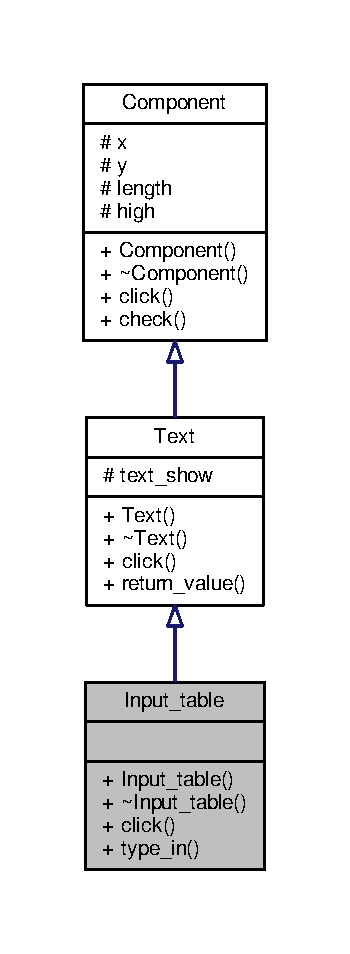
\includegraphics[width=168pt]{classInput__table__inherit__graph}
\end{center}
\end{figure}


Diagram współpracy dla Input\+\_\+table\+:\nopagebreak
\begin{figure}[H]
\begin{center}
\leavevmode
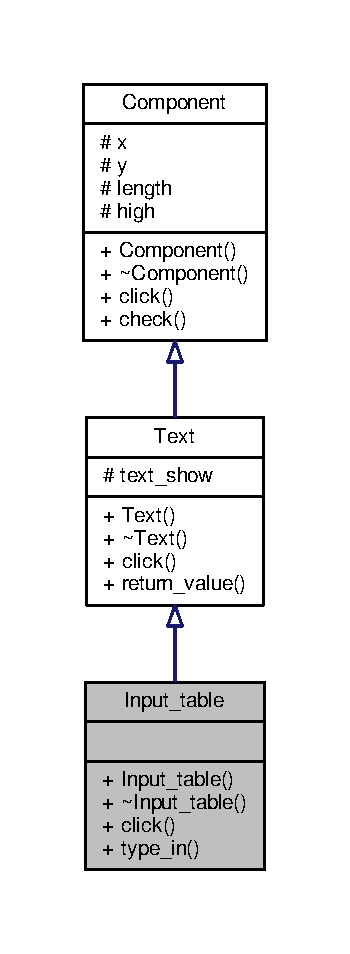
\includegraphics[width=168pt]{classInput__table__coll__graph}
\end{center}
\end{figure}
\subsection*{Metody publiczne}
\begin{DoxyCompactItemize}
\item 
\hyperlink{classInput__table_a45587a7a164f060d4bc10e30e2226e5d}{Input\+\_\+table} (int x\+\_\+axe=0, int y\+\_\+axe=0, int length\+\_\+p=30, int high\+\_\+p=10, string tekst\+\_\+p=\char`\"{}Type sentence\char`\"{})
\item 
\hyperlink{classInput__table_a22e1bdc68b3b830a03474b4897c6d47e}{$\sim$\+Input\+\_\+table} ()
\item 
virtual void \hyperlink{classInput__table_ac48806d103ed557c4b9a4eac4a021cf3}{click} ()
\item 
void \hyperlink{classInput__table_a6a4752b474d1a42c9f48bbb1e8af82a8}{type\+\_\+in} ()
\end{DoxyCompactItemize}
\subsection*{Dodatkowe Dziedziczone Składowe}


\subsection{Dokumentacja konstruktora i destruktora}
\index{Input\+\_\+table@{Input\+\_\+table}!Input\+\_\+table@{Input\+\_\+table}}
\index{Input\+\_\+table@{Input\+\_\+table}!Input\+\_\+table@{Input\+\_\+table}}
\subsubsection[{\texorpdfstring{Input\+\_\+table(int x\+\_\+axe=0, int y\+\_\+axe=0, int length\+\_\+p=30, int high\+\_\+p=10, string tekst\+\_\+p=""Type sentence"")}{Input_table(int x_axe=0, int y_axe=0, int length_p=30, int high_p=10, string tekst_p="Type sentence")}}]{\setlength{\rightskip}{0pt plus 5cm}Input\+\_\+table\+::\+Input\+\_\+table (
\begin{DoxyParamCaption}
\item[{int}]{x\+\_\+axe = {\ttfamily 0}, }
\item[{int}]{y\+\_\+axe = {\ttfamily 0}, }
\item[{int}]{length\+\_\+p = {\ttfamily 30}, }
\item[{int}]{high\+\_\+p = {\ttfamily 10}, }
\item[{string}]{tekst\+\_\+p = {\ttfamily \char`\"{}Type~sentence\char`\"{}}}
\end{DoxyParamCaption}
)\hspace{0.3cm}{\ttfamily [inline]}}\hypertarget{classInput__table_a45587a7a164f060d4bc10e30e2226e5d}{}\label{classInput__table_a45587a7a164f060d4bc10e30e2226e5d}
\index{Input\+\_\+table@{Input\+\_\+table}!````~Input\+\_\+table@{$\sim$\+Input\+\_\+table}}
\index{````~Input\+\_\+table@{$\sim$\+Input\+\_\+table}!Input\+\_\+table@{Input\+\_\+table}}
\subsubsection[{\texorpdfstring{$\sim$\+Input\+\_\+table()}{~Input_table()}}]{\setlength{\rightskip}{0pt plus 5cm}Input\+\_\+table\+::$\sim$\+Input\+\_\+table (
\begin{DoxyParamCaption}
{}
\end{DoxyParamCaption}
)\hspace{0.3cm}{\ttfamily [inline]}}\hypertarget{classInput__table_a22e1bdc68b3b830a03474b4897c6d47e}{}\label{classInput__table_a22e1bdc68b3b830a03474b4897c6d47e}


\subsection{Dokumentacja funkcji składowych}
\index{Input\+\_\+table@{Input\+\_\+table}!click@{click}}
\index{click@{click}!Input\+\_\+table@{Input\+\_\+table}}
\subsubsection[{\texorpdfstring{click()}{click()}}]{\setlength{\rightskip}{0pt plus 5cm}void Input\+\_\+table\+::click (
\begin{DoxyParamCaption}
{}
\end{DoxyParamCaption}
)\hspace{0.3cm}{\ttfamily [virtual]}}\hypertarget{classInput__table_ac48806d103ed557c4b9a4eac4a021cf3}{}\label{classInput__table_ac48806d103ed557c4b9a4eac4a021cf3}


Reimplementowana z \hyperlink{classText_ab334ff82f41302f83bebf3eaf2516a84}{Text}.

\index{Input\+\_\+table@{Input\+\_\+table}!type\+\_\+in@{type\+\_\+in}}
\index{type\+\_\+in@{type\+\_\+in}!Input\+\_\+table@{Input\+\_\+table}}
\subsubsection[{\texorpdfstring{type\+\_\+in()}{type_in()}}]{\setlength{\rightskip}{0pt plus 5cm}void Input\+\_\+table\+::type\+\_\+in (
\begin{DoxyParamCaption}
{}
\end{DoxyParamCaption}
)}\hypertarget{classInput__table_a6a4752b474d1a42c9f48bbb1e8af82a8}{}\label{classInput__table_a6a4752b474d1a42c9f48bbb1e8af82a8}


Dokumentacja dla tej klasy została wygenerowana z plików\+:\begin{DoxyCompactItemize}
\item 
\hyperlink{window_8h}{window.\+h}\item 
\hyperlink{window_8cpp}{window.\+cpp}\end{DoxyCompactItemize}

\hypertarget{classList}{}\section{Dokumentacja klasy List}
\label{classList}\index{List@{List}}


{\ttfamily \#include $<$window.\+h$>$}



Diagram dziedziczenia dla List
\nopagebreak
\begin{figure}[H]
\begin{center}
\leavevmode
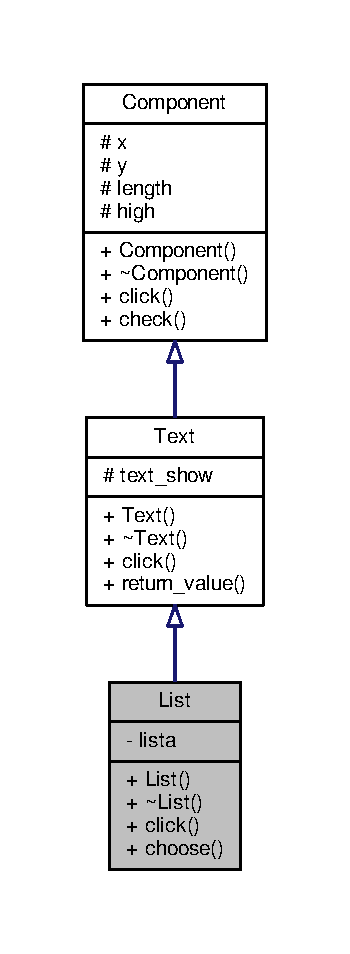
\includegraphics[width=168pt]{classList__inherit__graph}
\end{center}
\end{figure}


Diagram współpracy dla List\+:
\nopagebreak
\begin{figure}[H]
\begin{center}
\leavevmode
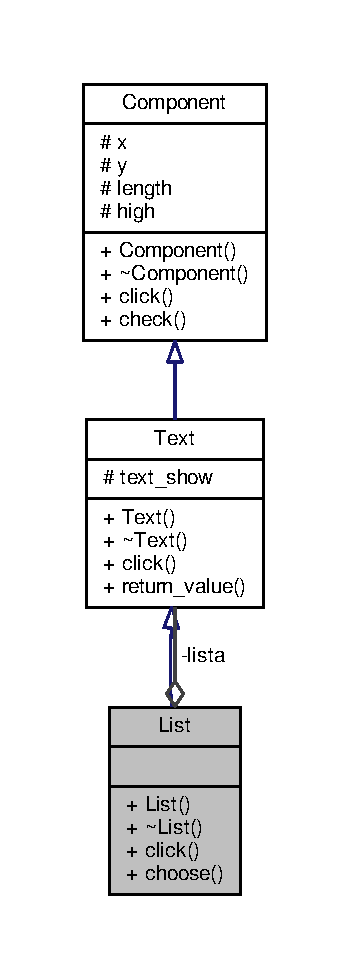
\includegraphics[width=168pt]{classList__coll__graph}
\end{center}
\end{figure}
\subsection*{Metody publiczne}
\begin{DoxyCompactItemize}
\item 
\hyperlink{classList_a461d7b92539ae6cd32801a93ef25c770}{List} (int x\+\_\+axe=0, int y\+\_\+axe=0, int length\+\_\+p=20, int high\+\_\+p=8, string tekst\+\_\+p=\char`\"{}Empty\char`\"{})
\item 
\hyperlink{classList_a70aecf37bd9d779a394e4d50377fbf5f}{$\sim$\+List} ()
\item 
virtual void \hyperlink{classList_a72af1f829c9b4ca5ee3cb3eaae52cf9a}{click} ()
\item 
void \hyperlink{classList_a0fd3881c847af3dd93bbc1927c2fff46}{choose} ()
\end{DoxyCompactItemize}
\subsection*{Atrybuty prywatne}
\begin{DoxyCompactItemize}
\item 
\hyperlink{classText}{Text} $\ast$ \hyperlink{classList_a1adf9a61f82738e8573517e24f915e79}{lista} \mbox{[}3\mbox{]}
\end{DoxyCompactItemize}
\subsection*{Dodatkowe Dziedziczone Składowe}


\subsection{Dokumentacja konstruktora i destruktora}
\index{List@{List}!List@{List}}
\index{List@{List}!List@{List}}
\subsubsection[{\texorpdfstring{List(int x\+\_\+axe=0, int y\+\_\+axe=0, int length\+\_\+p=20, int high\+\_\+p=8, string tekst\+\_\+p=""Empty"")}{List(int x_axe=0, int y_axe=0, int length_p=20, int high_p=8, string tekst_p="Empty")}}]{\setlength{\rightskip}{0pt plus 5cm}List\+::\+List (
\begin{DoxyParamCaption}
\item[{int}]{x\+\_\+axe = {\ttfamily 0}, }
\item[{int}]{y\+\_\+axe = {\ttfamily 0}, }
\item[{int}]{length\+\_\+p = {\ttfamily 20}, }
\item[{int}]{high\+\_\+p = {\ttfamily 8}, }
\item[{string}]{tekst\+\_\+p = {\ttfamily \char`\"{}Empty\char`\"{}}}
\end{DoxyParamCaption}
)\hspace{0.3cm}{\ttfamily [inline]}}\hypertarget{classList_a461d7b92539ae6cd32801a93ef25c770}{}\label{classList_a461d7b92539ae6cd32801a93ef25c770}
\index{List@{List}!````~List@{$\sim$\+List}}
\index{````~List@{$\sim$\+List}!List@{List}}
\subsubsection[{\texorpdfstring{$\sim$\+List()}{~List()}}]{\setlength{\rightskip}{0pt plus 5cm}List\+::$\sim$\+List (
\begin{DoxyParamCaption}
{}
\end{DoxyParamCaption}
)\hspace{0.3cm}{\ttfamily [inline]}}\hypertarget{classList_a70aecf37bd9d779a394e4d50377fbf5f}{}\label{classList_a70aecf37bd9d779a394e4d50377fbf5f}


\subsection{Dokumentacja funkcji składowych}
\index{List@{List}!choose@{choose}}
\index{choose@{choose}!List@{List}}
\subsubsection[{\texorpdfstring{choose()}{choose()}}]{\setlength{\rightskip}{0pt plus 5cm}void List\+::choose (
\begin{DoxyParamCaption}
{}
\end{DoxyParamCaption}
)}\hypertarget{classList_a0fd3881c847af3dd93bbc1927c2fff46}{}\label{classList_a0fd3881c847af3dd93bbc1927c2fff46}
\index{List@{List}!click@{click}}
\index{click@{click}!List@{List}}
\subsubsection[{\texorpdfstring{click()}{click()}}]{\setlength{\rightskip}{0pt plus 5cm}void List\+::click (
\begin{DoxyParamCaption}
{}
\end{DoxyParamCaption}
)\hspace{0.3cm}{\ttfamily [virtual]}}\hypertarget{classList_a72af1f829c9b4ca5ee3cb3eaae52cf9a}{}\label{classList_a72af1f829c9b4ca5ee3cb3eaae52cf9a}


Reimplementowana z \hyperlink{classText_ab334ff82f41302f83bebf3eaf2516a84}{Text}.



\subsection{Dokumentacja atrybutów składowych}
\index{List@{List}!lista@{lista}}
\index{lista@{lista}!List@{List}}
\subsubsection[{\texorpdfstring{lista}{lista}}]{\setlength{\rightskip}{0pt plus 5cm}{\bf Text}$\ast$ List\+::lista\mbox{[}3\mbox{]}\hspace{0.3cm}{\ttfamily [private]}}\hypertarget{classList_a1adf9a61f82738e8573517e24f915e79}{}\label{classList_a1adf9a61f82738e8573517e24f915e79}


Dokumentacja dla tej klasy została wygenerowana z plików\+:\begin{DoxyCompactItemize}
\item 
\hyperlink{window_8h}{window.\+h}\item 
\hyperlink{window_8cpp}{window.\+cpp}\end{DoxyCompactItemize}

\hypertarget{classText}{}\section{Dokumentacja klasy Text}
\label{classText}\index{Text@{Text}}


{\ttfamily \#include $<$window.\+h$>$}



Diagram dziedziczenia dla Text\nopagebreak
\begin{figure}[H]
\begin{center}
\leavevmode
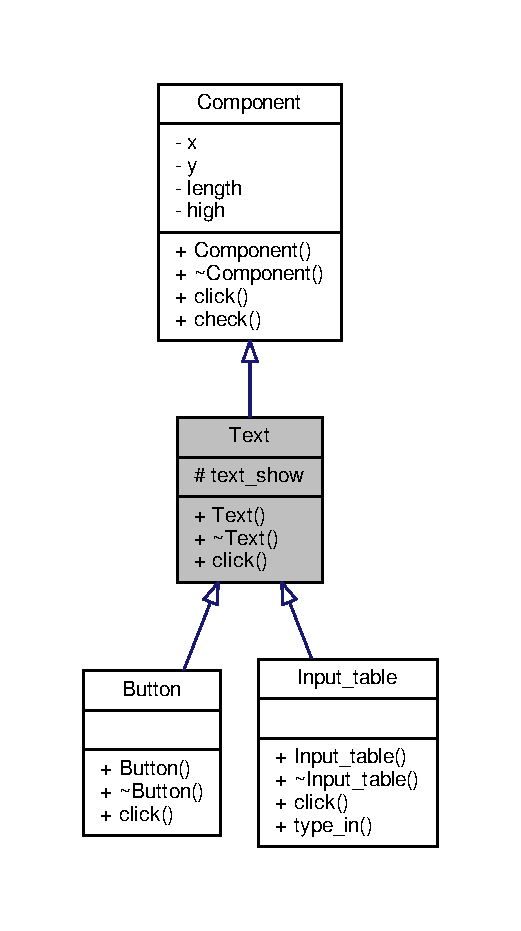
\includegraphics[width=350pt]{classText__inherit__graph}
\end{center}
\end{figure}


Diagram współpracy dla Text\+:\nopagebreak
\begin{figure}[H]
\begin{center}
\leavevmode
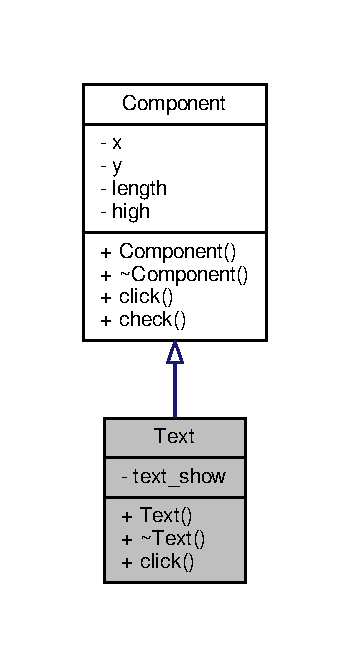
\includegraphics[width=168pt]{classText__coll__graph}
\end{center}
\end{figure}
\subsection*{Metody publiczne}
\begin{DoxyCompactItemize}
\item 
\hyperlink{classText_a144848b3b22ea514fe2f9c61762af5c3}{Text} (int x\+\_\+axe=0, int y\+\_\+axe=0, int length\+\_\+p=50, int high\+\_\+p=30, string text\+\_\+p=\char`\"{}Hello word!\char`\"{})
\item 
virtual \hyperlink{classText_a068e9e04751fc94f4c45c6cb15af55f4}{$\sim$\+Text} ()
\item 
virtual void \hyperlink{classText_ab334ff82f41302f83bebf3eaf2516a84}{click} ()
\end{DoxyCompactItemize}
\subsection*{Atrybuty prywatne}
\begin{DoxyCompactItemize}
\item 
string \hyperlink{classText_a3fd84b688c6971ba8626b910f0bc2ce3}{text\+\_\+show}
\end{DoxyCompactItemize}


\subsection{Dokumentacja konstruktora i destruktora}
\index{Text@{Text}!Text@{Text}}
\index{Text@{Text}!Text@{Text}}
\subsubsection[{\texorpdfstring{Text(int x\+\_\+axe=0, int y\+\_\+axe=0, int length\+\_\+p=50, int high\+\_\+p=30, string text\+\_\+p=""Hello word"!"")}{Text(int x_axe=0, int y_axe=0, int length_p=50, int high_p=30, string text_p="Hello word!")}}]{\setlength{\rightskip}{0pt plus 5cm}Text\+::\+Text (
\begin{DoxyParamCaption}
\item[{int}]{x\+\_\+axe = {\ttfamily 0}, }
\item[{int}]{y\+\_\+axe = {\ttfamily 0}, }
\item[{int}]{length\+\_\+p = {\ttfamily 50}, }
\item[{int}]{high\+\_\+p = {\ttfamily 30}, }
\item[{string}]{text\+\_\+p = {\ttfamily \char`\"{}Hello~word!\char`\"{}}}
\end{DoxyParamCaption}
)\hspace{0.3cm}{\ttfamily [inline]}}\hypertarget{classText_a144848b3b22ea514fe2f9c61762af5c3}{}\label{classText_a144848b3b22ea514fe2f9c61762af5c3}
\index{Text@{Text}!````~Text@{$\sim$\+Text}}
\index{````~Text@{$\sim$\+Text}!Text@{Text}}
\subsubsection[{\texorpdfstring{$\sim$\+Text()}{~Text()}}]{\setlength{\rightskip}{0pt plus 5cm}virtual Text\+::$\sim$\+Text (
\begin{DoxyParamCaption}
{}
\end{DoxyParamCaption}
)\hspace{0.3cm}{\ttfamily [inline]}, {\ttfamily [virtual]}}\hypertarget{classText_a068e9e04751fc94f4c45c6cb15af55f4}{}\label{classText_a068e9e04751fc94f4c45c6cb15af55f4}


\subsection{Dokumentacja funkcji składowych}
\index{Text@{Text}!click@{click}}
\index{click@{click}!Text@{Text}}
\subsubsection[{\texorpdfstring{click()}{click()}}]{\setlength{\rightskip}{0pt plus 5cm}void Text\+::click (
\begin{DoxyParamCaption}
{}
\end{DoxyParamCaption}
)\hspace{0.3cm}{\ttfamily [virtual]}}\hypertarget{classText_ab334ff82f41302f83bebf3eaf2516a84}{}\label{classText_ab334ff82f41302f83bebf3eaf2516a84}


Implementuje \hyperlink{classComponent_a247f6f0204b68a7efb9059cf709fe6ea}{Component}.



Reimplementowana w \hyperlink{classInput__table_ac48806d103ed557c4b9a4eac4a021cf3}{Input\+\_\+table}, \hyperlink{classCheckbox_afd75946a43da1dcba8e6f04f00df34ee}{Checkbox} i \hyperlink{classButton_a2fc33ec22217562b28ac6f02bda26c6e}{Button}.



\subsection{Dokumentacja atrybutów składowych}
\index{Text@{Text}!text\+\_\+show@{text\+\_\+show}}
\index{text\+\_\+show@{text\+\_\+show}!Text@{Text}}
\subsubsection[{\texorpdfstring{text\+\_\+show}{text_show}}]{\setlength{\rightskip}{0pt plus 5cm}string Text\+::text\+\_\+show\hspace{0.3cm}{\ttfamily [private]}}\hypertarget{classText_a3fd84b688c6971ba8626b910f0bc2ce3}{}\label{classText_a3fd84b688c6971ba8626b910f0bc2ce3}


Dokumentacja dla tej klasy została wygenerowana z plików\+:\begin{DoxyCompactItemize}
\item 
\hyperlink{window_8h}{window.\+h}\item 
\hyperlink{window_8cpp}{window.\+cpp}\end{DoxyCompactItemize}

\chapter{Dokumentacja plików}
\hypertarget{main_8cpp}{}\section{Dokumentacja pliku main.\+cpp}
\label{main_8cpp}\index{main.\+cpp@{main.\+cpp}}
{\ttfamily \#include $<$iostream$>$}\\*
{\ttfamily \#include \char`\"{}window.\+h\char`\"{}}\\*
{\ttfamily \#include \char`\"{}operating\+\_\+sys.\+h\char`\"{}}\\*
Wykres zależności załączania dla main.\+cpp\+:\nopagebreak
\begin{figure}[H]
\begin{center}
\leavevmode
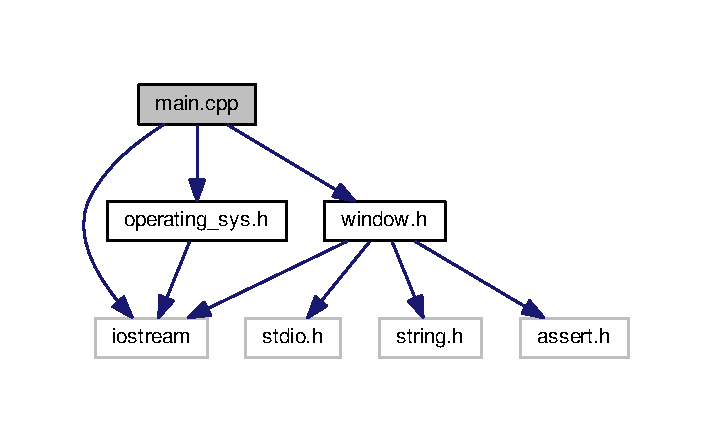
\includegraphics[width=342pt]{main_8cpp__incl}
\end{center}
\end{figure}
\subsection*{Funkcje}
\begin{DoxyCompactItemize}
\item 
int \hyperlink{main_8cpp_ae66f6b31b5ad750f1fe042a706a4e3d4}{main} ()
\end{DoxyCompactItemize}


\subsection{Dokumentacja funkcji}
\index{main.\+cpp@{main.\+cpp}!main@{main}}
\index{main@{main}!main.\+cpp@{main.\+cpp}}
\subsubsection[{\texorpdfstring{main()}{main()}}]{\setlength{\rightskip}{0pt plus 5cm}int main (
\begin{DoxyParamCaption}
{}
\end{DoxyParamCaption}
)}\hypertarget{main_8cpp_ae66f6b31b5ad750f1fe042a706a4e3d4}{}\label{main_8cpp_ae66f6b31b5ad750f1fe042a706a4e3d4}


Oto graf wywołań dla tej funkcji\+:\nopagebreak
\begin{figure}[H]
\begin{center}
\leavevmode
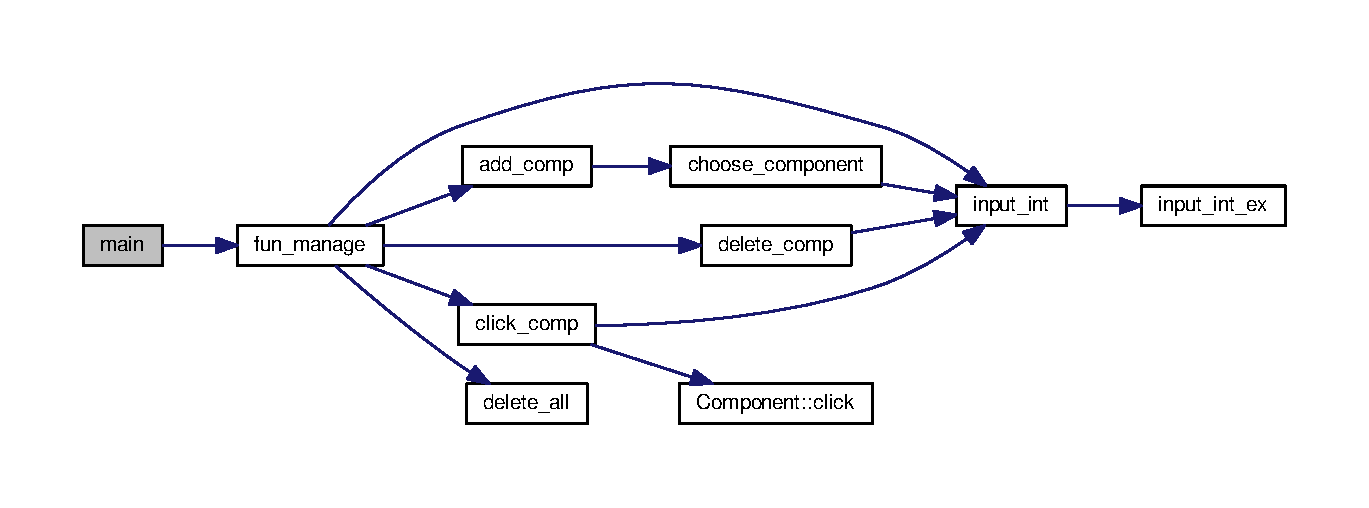
\includegraphics[width=350pt]{main_8cpp_ae66f6b31b5ad750f1fe042a706a4e3d4_cgraph}
\end{center}
\end{figure}



\hypertarget{operating__sys_8cpp}{}\section{Dokumentacja pliku operating\+\_\+sys.\+cpp}
\label{operating__sys_8cpp}\index{operating\+\_\+sys.\+cpp@{operating\+\_\+sys.\+cpp}}
{\ttfamily \#include $<$iostream$>$}\\*
{\ttfamily \#include $<$limits$>$}\\*
{\ttfamily \#include $<$stdio.\+h$>$}\\*
{\ttfamily \#include $<$string.\+h$>$}\\*
{\ttfamily \#include $<$vector$>$}\\*
{\ttfamily \#include $<$assert.\+h$>$}\\*
{\ttfamily \#include \char`\"{}window.\+h\char`\"{}}\\*
{\ttfamily \#include \char`\"{}operating\+\_\+sys.\+h\char`\"{}}\\*
Wykres zależności załączania dla operating\+\_\+sys.\+cpp\+:\nopagebreak
\begin{figure}[H]
\begin{center}
\leavevmode
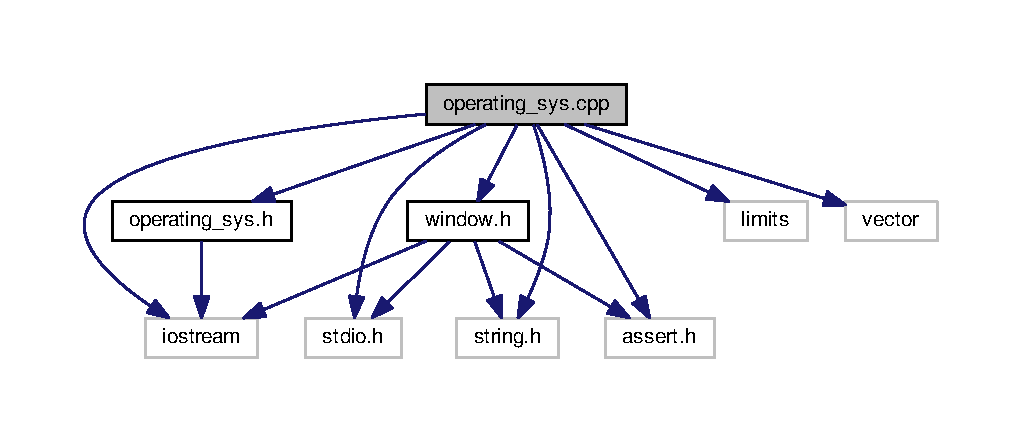
\includegraphics[width=350pt]{operating__sys_8cpp__incl}
\end{center}
\end{figure}
\subsection*{Funkcje}
\begin{DoxyCompactItemize}
\item 
void \hyperlink{operating__sys_8cpp_a1fb6c8e60497cc915d5bb21a1d2a3e8e}{input\+\_\+int\+\_\+ex} (int $\ast$ans)
\item 
int \hyperlink{operating__sys_8cpp_a3525598719638ffd3709dc4eb2be297c}{input\+\_\+int} ()
\item 
void \hyperlink{operating__sys_8cpp_a05f26d8f47cb9149d154961da6833924}{fun\+\_\+manage} ()
\item 
void \hyperlink{operating__sys_8cpp_ac92157a251599e7f5cdcccc80c8a4d8f}{add\+\_\+comp} ()
\item 
void \hyperlink{operating__sys_8cpp_a0dcf7e5b8c7e8248648160eedfb70be1}{choose\+\_\+component} ()
\item 
{\footnotesize template$<$class Typ $>$ }\\void \hyperlink{operating__sys_8cpp_a527d725cfb55d53a5a7db6226c06dd48}{create} ()
\item 
void \hyperlink{operating__sys_8cpp_a67f7d9237029a98ff5b20cf0f9d66f9c}{click\+\_\+comp} ()
\item 
void \hyperlink{operating__sys_8cpp_ae9ceeeedce8e1f1d1fd387f7b14b8342}{delete\+\_\+comp} ()
\item 
void \hyperlink{operating__sys_8cpp_a59d1ce49d7f44653c6a50e36166e2157}{delete\+\_\+all} ()
\end{DoxyCompactItemize}
\subsection*{Zmienne}
\begin{DoxyCompactItemize}
\item 
vector$<$ \hyperlink{classComponent}{Component} $\ast$ $>$ \hyperlink{operating__sys_8cpp_aeed90a084c9df14ccd76de382244e019}{data}
\item 
vector$<$ \hyperlink{classComponent}{Component} $\ast$ $>$\+::iterator \hyperlink{operating__sys_8cpp_a96b3c4c6338346ae5c84669a57f9eadb}{iter}
\end{DoxyCompactItemize}


\subsection{Dokumentacja funkcji}
\index{operating\+\_\+sys.\+cpp@{operating\+\_\+sys.\+cpp}!add\+\_\+comp@{add\+\_\+comp}}
\index{add\+\_\+comp@{add\+\_\+comp}!operating\+\_\+sys.\+cpp@{operating\+\_\+sys.\+cpp}}
\subsubsection[{\texorpdfstring{add\+\_\+comp()}{add_comp()}}]{\setlength{\rightskip}{0pt plus 5cm}void add\+\_\+comp (
\begin{DoxyParamCaption}
{}
\end{DoxyParamCaption}
)}\hypertarget{operating__sys_8cpp_ac92157a251599e7f5cdcccc80c8a4d8f}{}\label{operating__sys_8cpp_ac92157a251599e7f5cdcccc80c8a4d8f}


Oto graf wywołań dla tej funkcji\+:\nopagebreak
\begin{figure}[H]
\begin{center}
\leavevmode
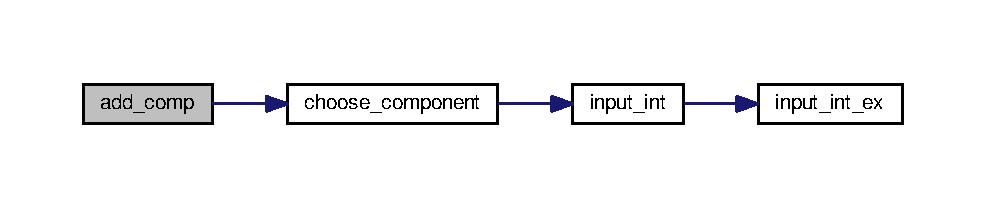
\includegraphics[width=350pt]{operating__sys_8cpp_ac92157a251599e7f5cdcccc80c8a4d8f_cgraph}
\end{center}
\end{figure}




Oto graf wywoływań tej funkcji\+:\nopagebreak
\begin{figure}[H]
\begin{center}
\leavevmode
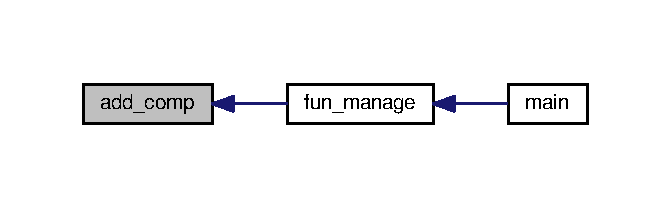
\includegraphics[width=322pt]{operating__sys_8cpp_ac92157a251599e7f5cdcccc80c8a4d8f_icgraph}
\end{center}
\end{figure}


\index{operating\+\_\+sys.\+cpp@{operating\+\_\+sys.\+cpp}!choose\+\_\+component@{choose\+\_\+component}}
\index{choose\+\_\+component@{choose\+\_\+component}!operating\+\_\+sys.\+cpp@{operating\+\_\+sys.\+cpp}}
\subsubsection[{\texorpdfstring{choose\+\_\+component()}{choose_component()}}]{\setlength{\rightskip}{0pt plus 5cm}void choose\+\_\+component (
\begin{DoxyParamCaption}
{}
\end{DoxyParamCaption}
)}\hypertarget{operating__sys_8cpp_a0dcf7e5b8c7e8248648160eedfb70be1}{}\label{operating__sys_8cpp_a0dcf7e5b8c7e8248648160eedfb70be1}


Oto graf wywołań dla tej funkcji\+:\nopagebreak
\begin{figure}[H]
\begin{center}
\leavevmode
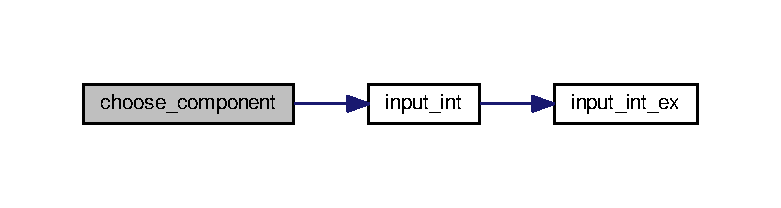
\includegraphics[width=350pt]{operating__sys_8cpp_a0dcf7e5b8c7e8248648160eedfb70be1_cgraph}
\end{center}
\end{figure}




Oto graf wywoływań tej funkcji\+:\nopagebreak
\begin{figure}[H]
\begin{center}
\leavevmode
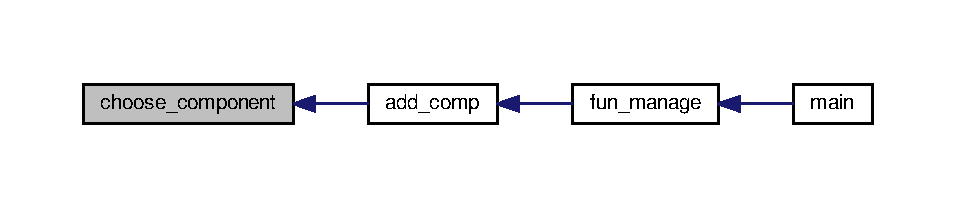
\includegraphics[width=350pt]{operating__sys_8cpp_a0dcf7e5b8c7e8248648160eedfb70be1_icgraph}
\end{center}
\end{figure}


\index{operating\+\_\+sys.\+cpp@{operating\+\_\+sys.\+cpp}!click\+\_\+comp@{click\+\_\+comp}}
\index{click\+\_\+comp@{click\+\_\+comp}!operating\+\_\+sys.\+cpp@{operating\+\_\+sys.\+cpp}}
\subsubsection[{\texorpdfstring{click\+\_\+comp()}{click_comp()}}]{\setlength{\rightskip}{0pt plus 5cm}void click\+\_\+comp (
\begin{DoxyParamCaption}
{}
\end{DoxyParamCaption}
)}\hypertarget{operating__sys_8cpp_a67f7d9237029a98ff5b20cf0f9d66f9c}{}\label{operating__sys_8cpp_a67f7d9237029a98ff5b20cf0f9d66f9c}


Oto graf wywołań dla tej funkcji\+:\nopagebreak
\begin{figure}[H]
\begin{center}
\leavevmode
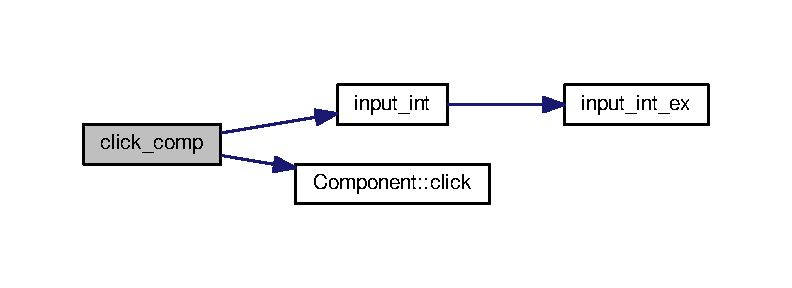
\includegraphics[width=350pt]{operating__sys_8cpp_a67f7d9237029a98ff5b20cf0f9d66f9c_cgraph}
\end{center}
\end{figure}




Oto graf wywoływań tej funkcji\+:\nopagebreak
\begin{figure}[H]
\begin{center}
\leavevmode
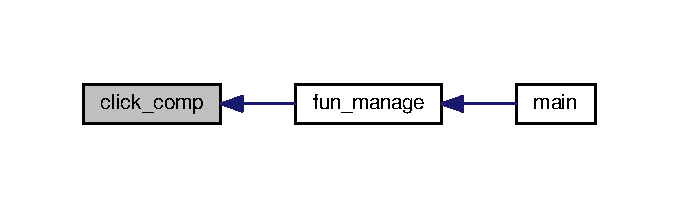
\includegraphics[width=326pt]{operating__sys_8cpp_a67f7d9237029a98ff5b20cf0f9d66f9c_icgraph}
\end{center}
\end{figure}


\index{operating\+\_\+sys.\+cpp@{operating\+\_\+sys.\+cpp}!create@{create}}
\index{create@{create}!operating\+\_\+sys.\+cpp@{operating\+\_\+sys.\+cpp}}
\subsubsection[{\texorpdfstring{create()}{create()}}]{\setlength{\rightskip}{0pt plus 5cm}template$<$class Typ $>$ void create (
\begin{DoxyParamCaption}
{}
\end{DoxyParamCaption}
)}\hypertarget{operating__sys_8cpp_a527d725cfb55d53a5a7db6226c06dd48}{}\label{operating__sys_8cpp_a527d725cfb55d53a5a7db6226c06dd48}


Oto graf wywołań dla tej funkcji\+:\nopagebreak
\begin{figure}[H]
\begin{center}
\leavevmode
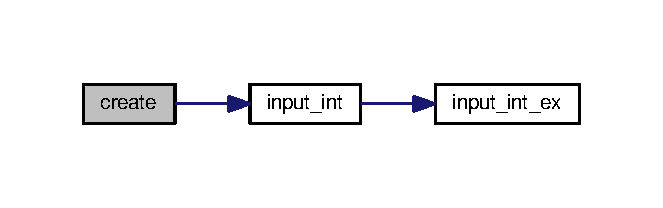
\includegraphics[width=318pt]{operating__sys_8cpp_a527d725cfb55d53a5a7db6226c06dd48_cgraph}
\end{center}
\end{figure}


\index{operating\+\_\+sys.\+cpp@{operating\+\_\+sys.\+cpp}!delete\+\_\+all@{delete\+\_\+all}}
\index{delete\+\_\+all@{delete\+\_\+all}!operating\+\_\+sys.\+cpp@{operating\+\_\+sys.\+cpp}}
\subsubsection[{\texorpdfstring{delete\+\_\+all()}{delete_all()}}]{\setlength{\rightskip}{0pt plus 5cm}void delete\+\_\+all (
\begin{DoxyParamCaption}
{}
\end{DoxyParamCaption}
)}\hypertarget{operating__sys_8cpp_a59d1ce49d7f44653c6a50e36166e2157}{}\label{operating__sys_8cpp_a59d1ce49d7f44653c6a50e36166e2157}


Oto graf wywoływań tej funkcji\+:\nopagebreak
\begin{figure}[H]
\begin{center}
\leavevmode
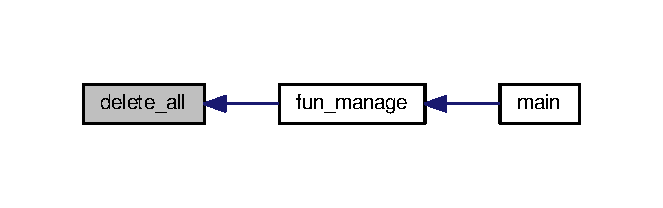
\includegraphics[width=318pt]{operating__sys_8cpp_a59d1ce49d7f44653c6a50e36166e2157_icgraph}
\end{center}
\end{figure}


\index{operating\+\_\+sys.\+cpp@{operating\+\_\+sys.\+cpp}!delete\+\_\+comp@{delete\+\_\+comp}}
\index{delete\+\_\+comp@{delete\+\_\+comp}!operating\+\_\+sys.\+cpp@{operating\+\_\+sys.\+cpp}}
\subsubsection[{\texorpdfstring{delete\+\_\+comp()}{delete_comp()}}]{\setlength{\rightskip}{0pt plus 5cm}void delete\+\_\+comp (
\begin{DoxyParamCaption}
{}
\end{DoxyParamCaption}
)}\hypertarget{operating__sys_8cpp_ae9ceeeedce8e1f1d1fd387f7b14b8342}{}\label{operating__sys_8cpp_ae9ceeeedce8e1f1d1fd387f7b14b8342}


Oto graf wywołań dla tej funkcji\+:\nopagebreak
\begin{figure}[H]
\begin{center}
\leavevmode
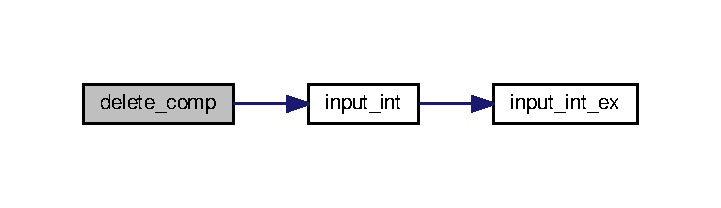
\includegraphics[width=346pt]{operating__sys_8cpp_ae9ceeeedce8e1f1d1fd387f7b14b8342_cgraph}
\end{center}
\end{figure}




Oto graf wywoływań tej funkcji\+:\nopagebreak
\begin{figure}[H]
\begin{center}
\leavevmode
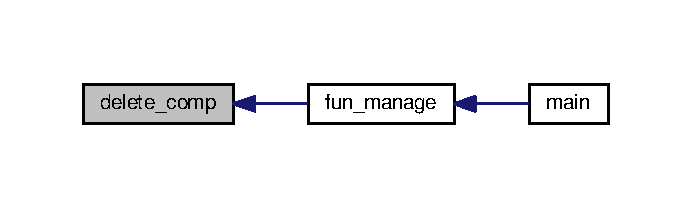
\includegraphics[width=332pt]{operating__sys_8cpp_ae9ceeeedce8e1f1d1fd387f7b14b8342_icgraph}
\end{center}
\end{figure}


\index{operating\+\_\+sys.\+cpp@{operating\+\_\+sys.\+cpp}!fun\+\_\+manage@{fun\+\_\+manage}}
\index{fun\+\_\+manage@{fun\+\_\+manage}!operating\+\_\+sys.\+cpp@{operating\+\_\+sys.\+cpp}}
\subsubsection[{\texorpdfstring{fun\+\_\+manage()}{fun_manage()}}]{\setlength{\rightskip}{0pt plus 5cm}void fun\+\_\+manage (
\begin{DoxyParamCaption}
{}
\end{DoxyParamCaption}
)}\hypertarget{operating__sys_8cpp_a05f26d8f47cb9149d154961da6833924}{}\label{operating__sys_8cpp_a05f26d8f47cb9149d154961da6833924}


Oto graf wywołań dla tej funkcji\+:\nopagebreak
\begin{figure}[H]
\begin{center}
\leavevmode
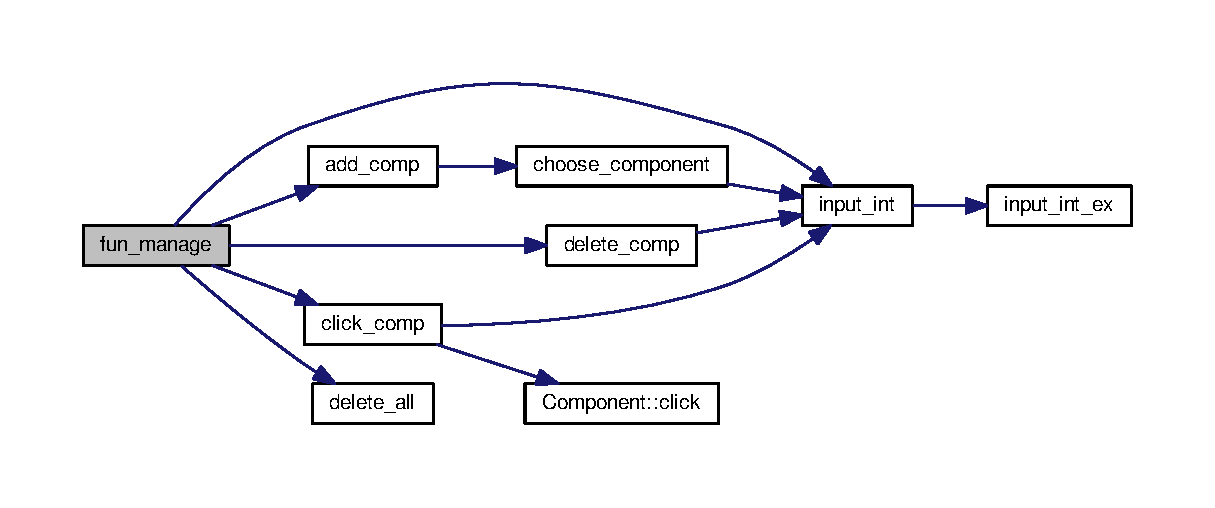
\includegraphics[width=350pt]{operating__sys_8cpp_a05f26d8f47cb9149d154961da6833924_cgraph}
\end{center}
\end{figure}




Oto graf wywoływań tej funkcji\+:\nopagebreak
\begin{figure}[H]
\begin{center}
\leavevmode
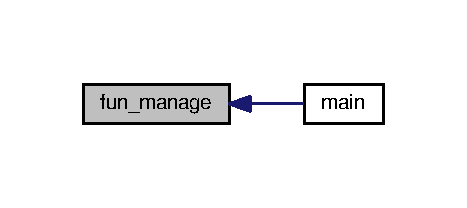
\includegraphics[width=224pt]{operating__sys_8cpp_a05f26d8f47cb9149d154961da6833924_icgraph}
\end{center}
\end{figure}


\index{operating\+\_\+sys.\+cpp@{operating\+\_\+sys.\+cpp}!input\+\_\+int@{input\+\_\+int}}
\index{input\+\_\+int@{input\+\_\+int}!operating\+\_\+sys.\+cpp@{operating\+\_\+sys.\+cpp}}
\subsubsection[{\texorpdfstring{input\+\_\+int()}{input_int()}}]{\setlength{\rightskip}{0pt plus 5cm}int input\+\_\+int (
\begin{DoxyParamCaption}
{}
\end{DoxyParamCaption}
)}\hypertarget{operating__sys_8cpp_a3525598719638ffd3709dc4eb2be297c}{}\label{operating__sys_8cpp_a3525598719638ffd3709dc4eb2be297c}


Oto graf wywołań dla tej funkcji\+:\nopagebreak
\begin{figure}[H]
\begin{center}
\leavevmode
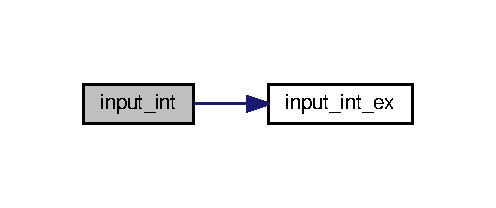
\includegraphics[width=238pt]{operating__sys_8cpp_a3525598719638ffd3709dc4eb2be297c_cgraph}
\end{center}
\end{figure}




Oto graf wywoływań tej funkcji\+:\nopagebreak
\begin{figure}[H]
\begin{center}
\leavevmode
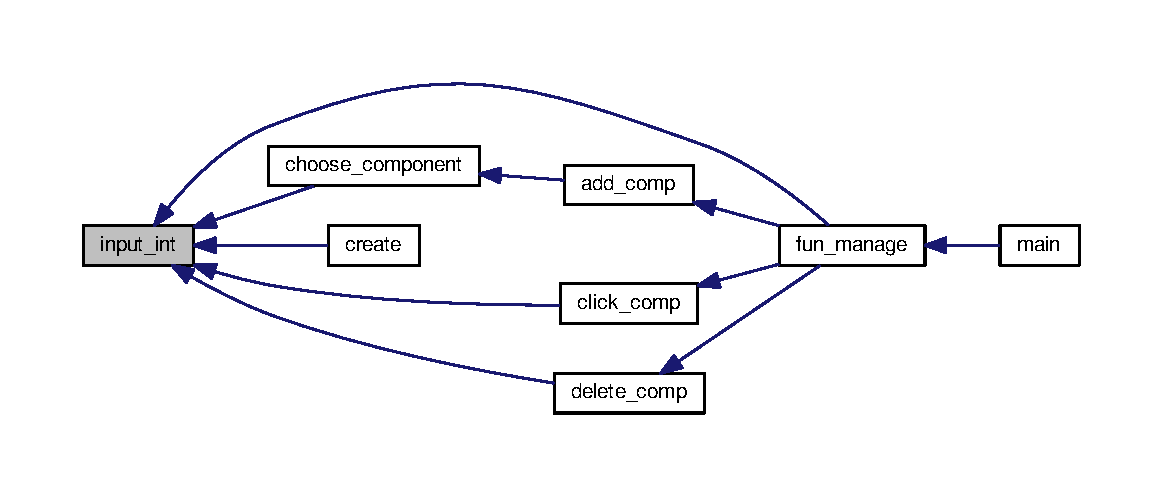
\includegraphics[width=350pt]{operating__sys_8cpp_a3525598719638ffd3709dc4eb2be297c_icgraph}
\end{center}
\end{figure}


\index{operating\+\_\+sys.\+cpp@{operating\+\_\+sys.\+cpp}!input\+\_\+int\+\_\+ex@{input\+\_\+int\+\_\+ex}}
\index{input\+\_\+int\+\_\+ex@{input\+\_\+int\+\_\+ex}!operating\+\_\+sys.\+cpp@{operating\+\_\+sys.\+cpp}}
\subsubsection[{\texorpdfstring{input\+\_\+int\+\_\+ex(int $\ast$ans)}{input_int_ex(int *ans)}}]{\setlength{\rightskip}{0pt plus 5cm}void input\+\_\+int\+\_\+ex (
\begin{DoxyParamCaption}
\item[{int $\ast$}]{ans}
\end{DoxyParamCaption}
)}\hypertarget{operating__sys_8cpp_a1fb6c8e60497cc915d5bb21a1d2a3e8e}{}\label{operating__sys_8cpp_a1fb6c8e60497cc915d5bb21a1d2a3e8e}


Oto graf wywoływań tej funkcji\+:\nopagebreak
\begin{figure}[H]
\begin{center}
\leavevmode
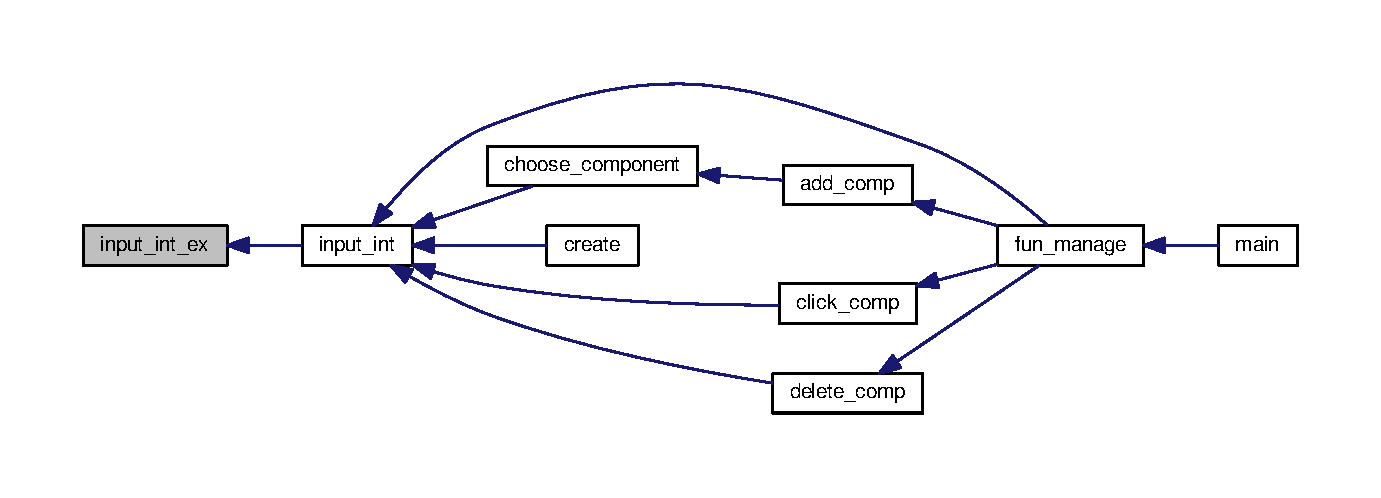
\includegraphics[width=350pt]{operating__sys_8cpp_a1fb6c8e60497cc915d5bb21a1d2a3e8e_icgraph}
\end{center}
\end{figure}




\subsection{Dokumentacja zmiennych}
\index{operating\+\_\+sys.\+cpp@{operating\+\_\+sys.\+cpp}!data@{data}}
\index{data@{data}!operating\+\_\+sys.\+cpp@{operating\+\_\+sys.\+cpp}}
\subsubsection[{\texorpdfstring{data}{data}}]{\setlength{\rightskip}{0pt plus 5cm}vector$<${\bf Component}$\ast$$>$ data}\hypertarget{operating__sys_8cpp_aeed90a084c9df14ccd76de382244e019}{}\label{operating__sys_8cpp_aeed90a084c9df14ccd76de382244e019}
\index{operating\+\_\+sys.\+cpp@{operating\+\_\+sys.\+cpp}!iter@{iter}}
\index{iter@{iter}!operating\+\_\+sys.\+cpp@{operating\+\_\+sys.\+cpp}}
\subsubsection[{\texorpdfstring{iter}{iter}}]{\setlength{\rightskip}{0pt plus 5cm}vector$<${\bf Component}$\ast$$>$\+::iterator iter}\hypertarget{operating__sys_8cpp_a96b3c4c6338346ae5c84669a57f9eadb}{}\label{operating__sys_8cpp_a96b3c4c6338346ae5c84669a57f9eadb}

\hypertarget{operating__sys_8h}{}\section{Dokumentacja pliku operating\+\_\+sys.\+h}
\label{operating__sys_8h}\index{operating\+\_\+sys.\+h@{operating\+\_\+sys.\+h}}
{\ttfamily \#include $<$iostream$>$}\\*
Wykres zależności załączania dla operating\+\_\+sys.\+h\+:\nopagebreak
\begin{figure}[H]
\begin{center}
\leavevmode
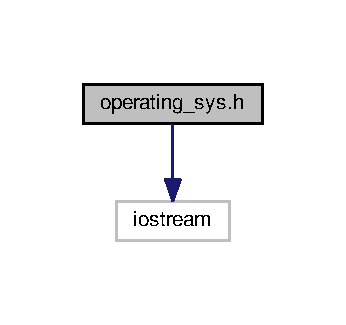
\includegraphics[width=166pt]{operating__sys_8h__incl}
\end{center}
\end{figure}
Ten wykres pokazuje, które pliki bezpośrednio lub pośrednio załączają ten plik\+:\nopagebreak
\begin{figure}[H]
\begin{center}
\leavevmode
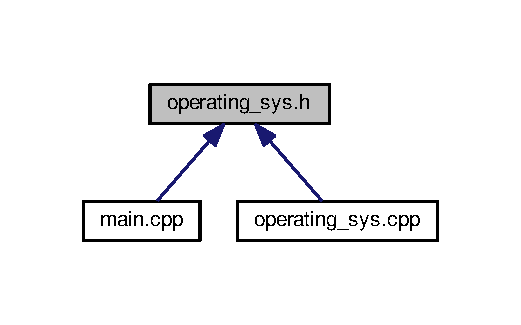
\includegraphics[width=250pt]{operating__sys_8h__dep__incl}
\end{center}
\end{figure}
\subsection*{Funkcje}
\begin{DoxyCompactItemize}
\item 
int \hyperlink{operating__sys_8h_a3525598719638ffd3709dc4eb2be297c}{input\+\_\+int} ()
\item 
void \hyperlink{operating__sys_8h_a1fb6c8e60497cc915d5bb21a1d2a3e8e}{input\+\_\+int\+\_\+ex} (int $\ast$ans)
\item 
void \hyperlink{operating__sys_8h_a0dcf7e5b8c7e8248648160eedfb70be1}{choose\+\_\+component} ()
\item 
void \hyperlink{operating__sys_8h_ac92157a251599e7f5cdcccc80c8a4d8f}{add\+\_\+comp} ()
\item 
{\footnotesize template$<$class Typ $>$ }\\void \hyperlink{operating__sys_8h_a527d725cfb55d53a5a7db6226c06dd48}{create} ()
\item 
void \hyperlink{operating__sys_8h_ae9ceeeedce8e1f1d1fd387f7b14b8342}{delete\+\_\+comp} ()
\item 
void \hyperlink{operating__sys_8h_a59d1ce49d7f44653c6a50e36166e2157}{delete\+\_\+all} ()
\item 
void \hyperlink{operating__sys_8h_a67f7d9237029a98ff5b20cf0f9d66f9c}{click\+\_\+comp} ()
\item 
void \hyperlink{operating__sys_8h_a05f26d8f47cb9149d154961da6833924}{fun\+\_\+manage} ()
\end{DoxyCompactItemize}


\subsection{Dokumentacja funkcji}
\index{operating\+\_\+sys.\+h@{operating\+\_\+sys.\+h}!add\+\_\+comp@{add\+\_\+comp}}
\index{add\+\_\+comp@{add\+\_\+comp}!operating\+\_\+sys.\+h@{operating\+\_\+sys.\+h}}
\subsubsection[{\texorpdfstring{add\+\_\+comp()}{add_comp()}}]{\setlength{\rightskip}{0pt plus 5cm}void add\+\_\+comp (
\begin{DoxyParamCaption}
{}
\end{DoxyParamCaption}
)}\hypertarget{operating__sys_8h_ac92157a251599e7f5cdcccc80c8a4d8f}{}\label{operating__sys_8h_ac92157a251599e7f5cdcccc80c8a4d8f}


Oto graf wywołań dla tej funkcji\+:\nopagebreak
\begin{figure}[H]
\begin{center}
\leavevmode
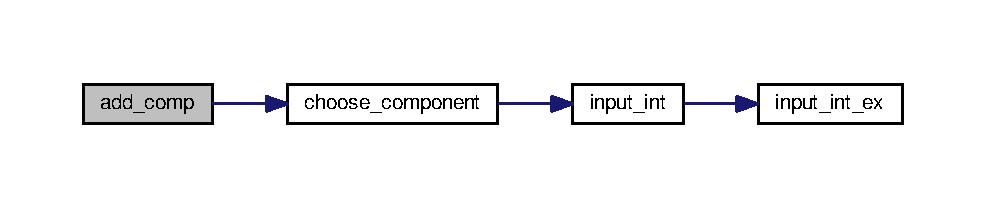
\includegraphics[width=350pt]{operating__sys_8h_ac92157a251599e7f5cdcccc80c8a4d8f_cgraph}
\end{center}
\end{figure}




Oto graf wywoływań tej funkcji\+:\nopagebreak
\begin{figure}[H]
\begin{center}
\leavevmode
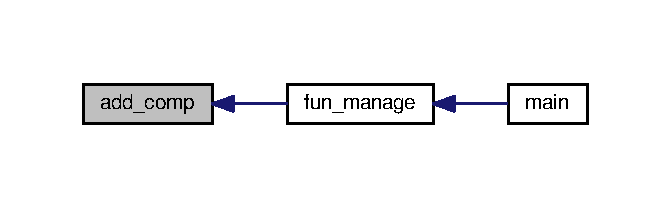
\includegraphics[width=322pt]{operating__sys_8h_ac92157a251599e7f5cdcccc80c8a4d8f_icgraph}
\end{center}
\end{figure}


\index{operating\+\_\+sys.\+h@{operating\+\_\+sys.\+h}!choose\+\_\+component@{choose\+\_\+component}}
\index{choose\+\_\+component@{choose\+\_\+component}!operating\+\_\+sys.\+h@{operating\+\_\+sys.\+h}}
\subsubsection[{\texorpdfstring{choose\+\_\+component()}{choose_component()}}]{\setlength{\rightskip}{0pt plus 5cm}void choose\+\_\+component (
\begin{DoxyParamCaption}
{}
\end{DoxyParamCaption}
)}\hypertarget{operating__sys_8h_a0dcf7e5b8c7e8248648160eedfb70be1}{}\label{operating__sys_8h_a0dcf7e5b8c7e8248648160eedfb70be1}


Oto graf wywołań dla tej funkcji\+:\nopagebreak
\begin{figure}[H]
\begin{center}
\leavevmode
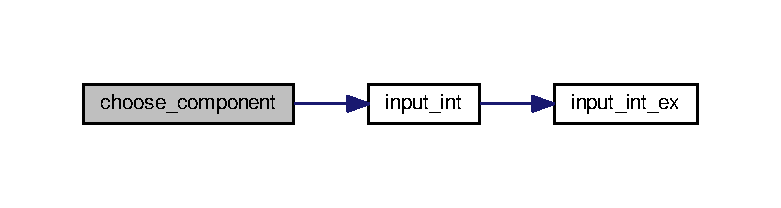
\includegraphics[width=350pt]{operating__sys_8h_a0dcf7e5b8c7e8248648160eedfb70be1_cgraph}
\end{center}
\end{figure}




Oto graf wywoływań tej funkcji\+:\nopagebreak
\begin{figure}[H]
\begin{center}
\leavevmode
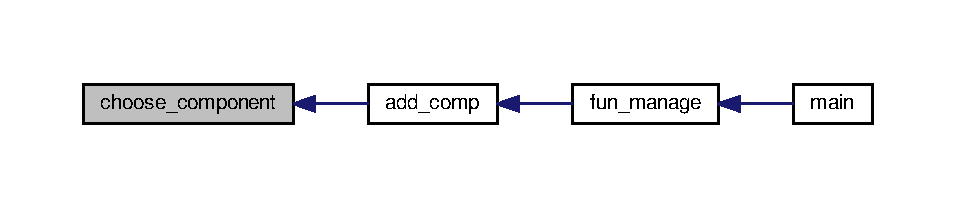
\includegraphics[width=350pt]{operating__sys_8h_a0dcf7e5b8c7e8248648160eedfb70be1_icgraph}
\end{center}
\end{figure}


\index{operating\+\_\+sys.\+h@{operating\+\_\+sys.\+h}!click\+\_\+comp@{click\+\_\+comp}}
\index{click\+\_\+comp@{click\+\_\+comp}!operating\+\_\+sys.\+h@{operating\+\_\+sys.\+h}}
\subsubsection[{\texorpdfstring{click\+\_\+comp()}{click_comp()}}]{\setlength{\rightskip}{0pt plus 5cm}void click\+\_\+comp (
\begin{DoxyParamCaption}
{}
\end{DoxyParamCaption}
)}\hypertarget{operating__sys_8h_a67f7d9237029a98ff5b20cf0f9d66f9c}{}\label{operating__sys_8h_a67f7d9237029a98ff5b20cf0f9d66f9c}


Oto graf wywołań dla tej funkcji\+:\nopagebreak
\begin{figure}[H]
\begin{center}
\leavevmode
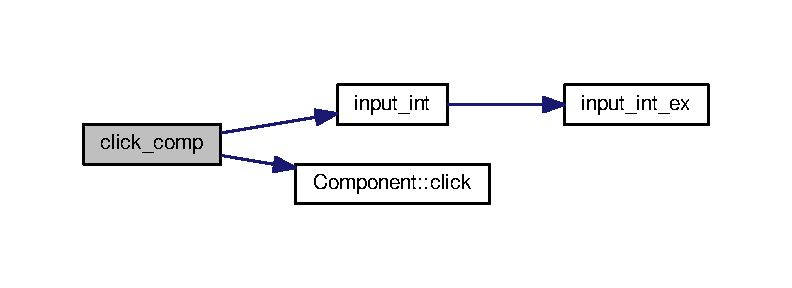
\includegraphics[width=350pt]{operating__sys_8h_a67f7d9237029a98ff5b20cf0f9d66f9c_cgraph}
\end{center}
\end{figure}




Oto graf wywoływań tej funkcji\+:\nopagebreak
\begin{figure}[H]
\begin{center}
\leavevmode
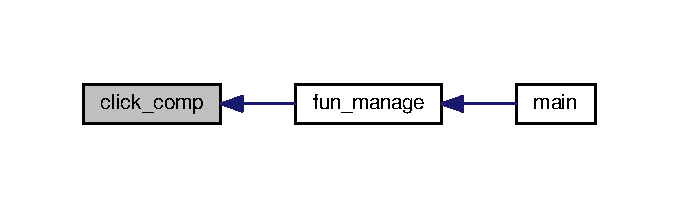
\includegraphics[width=326pt]{operating__sys_8h_a67f7d9237029a98ff5b20cf0f9d66f9c_icgraph}
\end{center}
\end{figure}


\index{operating\+\_\+sys.\+h@{operating\+\_\+sys.\+h}!create@{create}}
\index{create@{create}!operating\+\_\+sys.\+h@{operating\+\_\+sys.\+h}}
\subsubsection[{\texorpdfstring{create()}{create()}}]{\setlength{\rightskip}{0pt plus 5cm}template$<$class Typ $>$ void create (
\begin{DoxyParamCaption}
{}
\end{DoxyParamCaption}
)}\hypertarget{operating__sys_8h_a527d725cfb55d53a5a7db6226c06dd48}{}\label{operating__sys_8h_a527d725cfb55d53a5a7db6226c06dd48}


Oto graf wywołań dla tej funkcji\+:\nopagebreak
\begin{figure}[H]
\begin{center}
\leavevmode
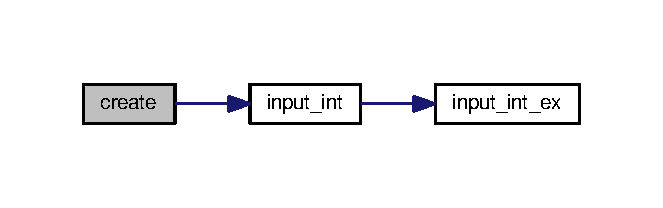
\includegraphics[width=318pt]{operating__sys_8h_a527d725cfb55d53a5a7db6226c06dd48_cgraph}
\end{center}
\end{figure}


\index{operating\+\_\+sys.\+h@{operating\+\_\+sys.\+h}!delete\+\_\+all@{delete\+\_\+all}}
\index{delete\+\_\+all@{delete\+\_\+all}!operating\+\_\+sys.\+h@{operating\+\_\+sys.\+h}}
\subsubsection[{\texorpdfstring{delete\+\_\+all()}{delete_all()}}]{\setlength{\rightskip}{0pt plus 5cm}void delete\+\_\+all (
\begin{DoxyParamCaption}
{}
\end{DoxyParamCaption}
)}\hypertarget{operating__sys_8h_a59d1ce49d7f44653c6a50e36166e2157}{}\label{operating__sys_8h_a59d1ce49d7f44653c6a50e36166e2157}


Oto graf wywoływań tej funkcji\+:\nopagebreak
\begin{figure}[H]
\begin{center}
\leavevmode
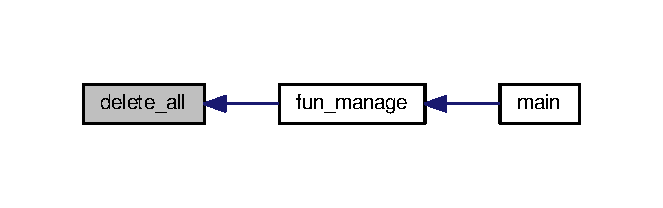
\includegraphics[width=318pt]{operating__sys_8h_a59d1ce49d7f44653c6a50e36166e2157_icgraph}
\end{center}
\end{figure}


\index{operating\+\_\+sys.\+h@{operating\+\_\+sys.\+h}!delete\+\_\+comp@{delete\+\_\+comp}}
\index{delete\+\_\+comp@{delete\+\_\+comp}!operating\+\_\+sys.\+h@{operating\+\_\+sys.\+h}}
\subsubsection[{\texorpdfstring{delete\+\_\+comp()}{delete_comp()}}]{\setlength{\rightskip}{0pt plus 5cm}void delete\+\_\+comp (
\begin{DoxyParamCaption}
{}
\end{DoxyParamCaption}
)}\hypertarget{operating__sys_8h_ae9ceeeedce8e1f1d1fd387f7b14b8342}{}\label{operating__sys_8h_ae9ceeeedce8e1f1d1fd387f7b14b8342}


Oto graf wywołań dla tej funkcji\+:\nopagebreak
\begin{figure}[H]
\begin{center}
\leavevmode
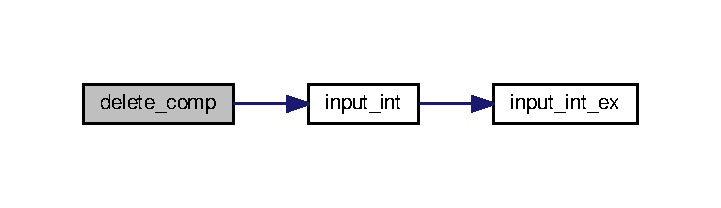
\includegraphics[width=346pt]{operating__sys_8h_ae9ceeeedce8e1f1d1fd387f7b14b8342_cgraph}
\end{center}
\end{figure}




Oto graf wywoływań tej funkcji\+:\nopagebreak
\begin{figure}[H]
\begin{center}
\leavevmode
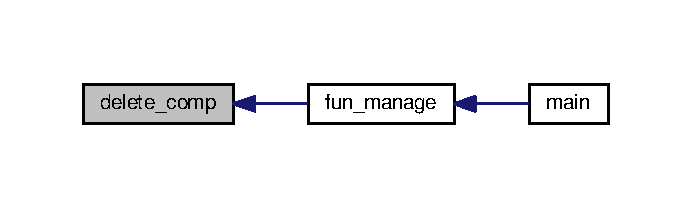
\includegraphics[width=332pt]{operating__sys_8h_ae9ceeeedce8e1f1d1fd387f7b14b8342_icgraph}
\end{center}
\end{figure}


\index{operating\+\_\+sys.\+h@{operating\+\_\+sys.\+h}!fun\+\_\+manage@{fun\+\_\+manage}}
\index{fun\+\_\+manage@{fun\+\_\+manage}!operating\+\_\+sys.\+h@{operating\+\_\+sys.\+h}}
\subsubsection[{\texorpdfstring{fun\+\_\+manage()}{fun_manage()}}]{\setlength{\rightskip}{0pt plus 5cm}void fun\+\_\+manage (
\begin{DoxyParamCaption}
{}
\end{DoxyParamCaption}
)}\hypertarget{operating__sys_8h_a05f26d8f47cb9149d154961da6833924}{}\label{operating__sys_8h_a05f26d8f47cb9149d154961da6833924}


Oto graf wywołań dla tej funkcji\+:\nopagebreak
\begin{figure}[H]
\begin{center}
\leavevmode
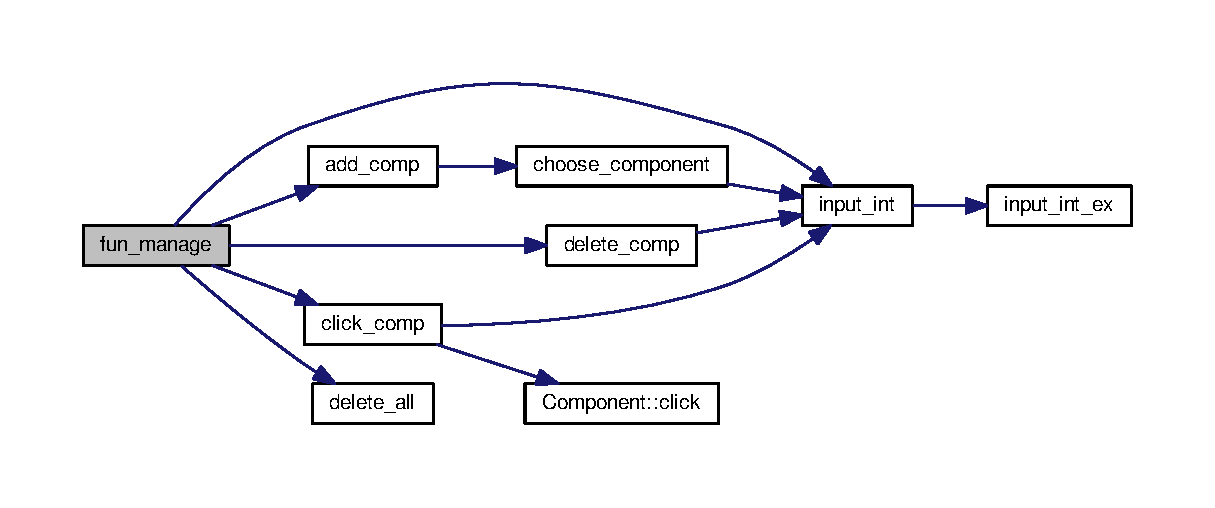
\includegraphics[width=350pt]{operating__sys_8h_a05f26d8f47cb9149d154961da6833924_cgraph}
\end{center}
\end{figure}




Oto graf wywoływań tej funkcji\+:\nopagebreak
\begin{figure}[H]
\begin{center}
\leavevmode
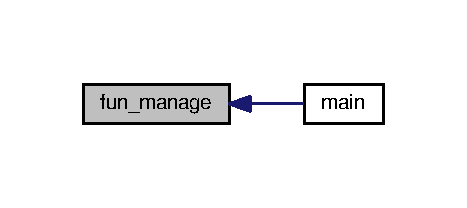
\includegraphics[width=224pt]{operating__sys_8h_a05f26d8f47cb9149d154961da6833924_icgraph}
\end{center}
\end{figure}


\index{operating\+\_\+sys.\+h@{operating\+\_\+sys.\+h}!input\+\_\+int@{input\+\_\+int}}
\index{input\+\_\+int@{input\+\_\+int}!operating\+\_\+sys.\+h@{operating\+\_\+sys.\+h}}
\subsubsection[{\texorpdfstring{input\+\_\+int()}{input_int()}}]{\setlength{\rightskip}{0pt plus 5cm}int input\+\_\+int (
\begin{DoxyParamCaption}
{}
\end{DoxyParamCaption}
)}\hypertarget{operating__sys_8h_a3525598719638ffd3709dc4eb2be297c}{}\label{operating__sys_8h_a3525598719638ffd3709dc4eb2be297c}


Oto graf wywołań dla tej funkcji\+:\nopagebreak
\begin{figure}[H]
\begin{center}
\leavevmode
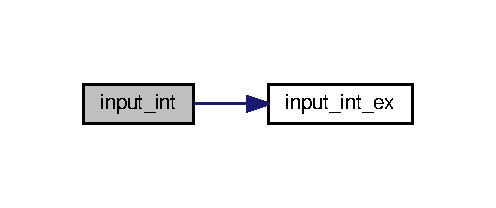
\includegraphics[width=238pt]{operating__sys_8h_a3525598719638ffd3709dc4eb2be297c_cgraph}
\end{center}
\end{figure}




Oto graf wywoływań tej funkcji\+:\nopagebreak
\begin{figure}[H]
\begin{center}
\leavevmode
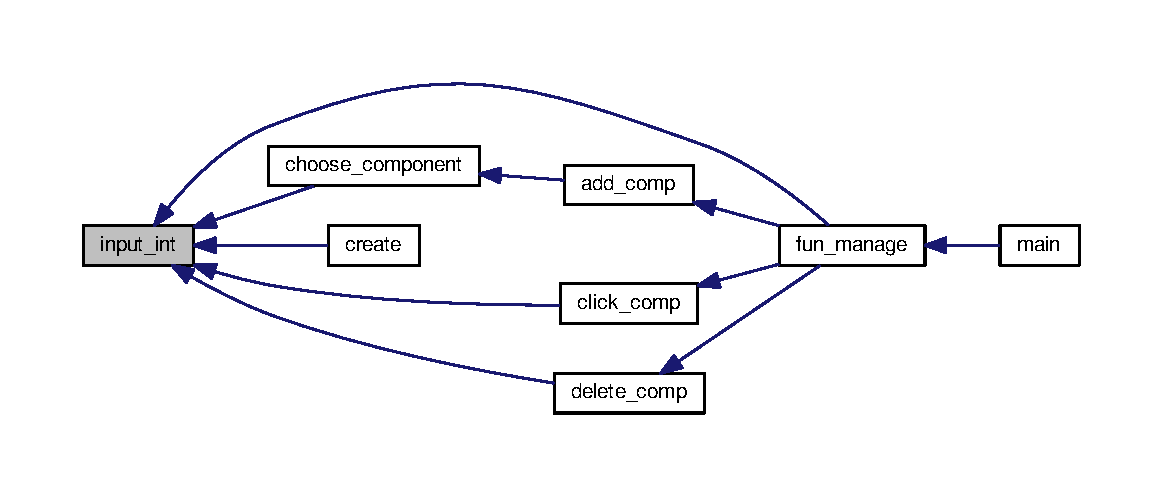
\includegraphics[width=350pt]{operating__sys_8h_a3525598719638ffd3709dc4eb2be297c_icgraph}
\end{center}
\end{figure}


\index{operating\+\_\+sys.\+h@{operating\+\_\+sys.\+h}!input\+\_\+int\+\_\+ex@{input\+\_\+int\+\_\+ex}}
\index{input\+\_\+int\+\_\+ex@{input\+\_\+int\+\_\+ex}!operating\+\_\+sys.\+h@{operating\+\_\+sys.\+h}}
\subsubsection[{\texorpdfstring{input\+\_\+int\+\_\+ex(int $\ast$ans)}{input_int_ex(int *ans)}}]{\setlength{\rightskip}{0pt plus 5cm}void input\+\_\+int\+\_\+ex (
\begin{DoxyParamCaption}
\item[{int $\ast$}]{ans}
\end{DoxyParamCaption}
)}\hypertarget{operating__sys_8h_a1fb6c8e60497cc915d5bb21a1d2a3e8e}{}\label{operating__sys_8h_a1fb6c8e60497cc915d5bb21a1d2a3e8e}


Oto graf wywoływań tej funkcji\+:\nopagebreak
\begin{figure}[H]
\begin{center}
\leavevmode
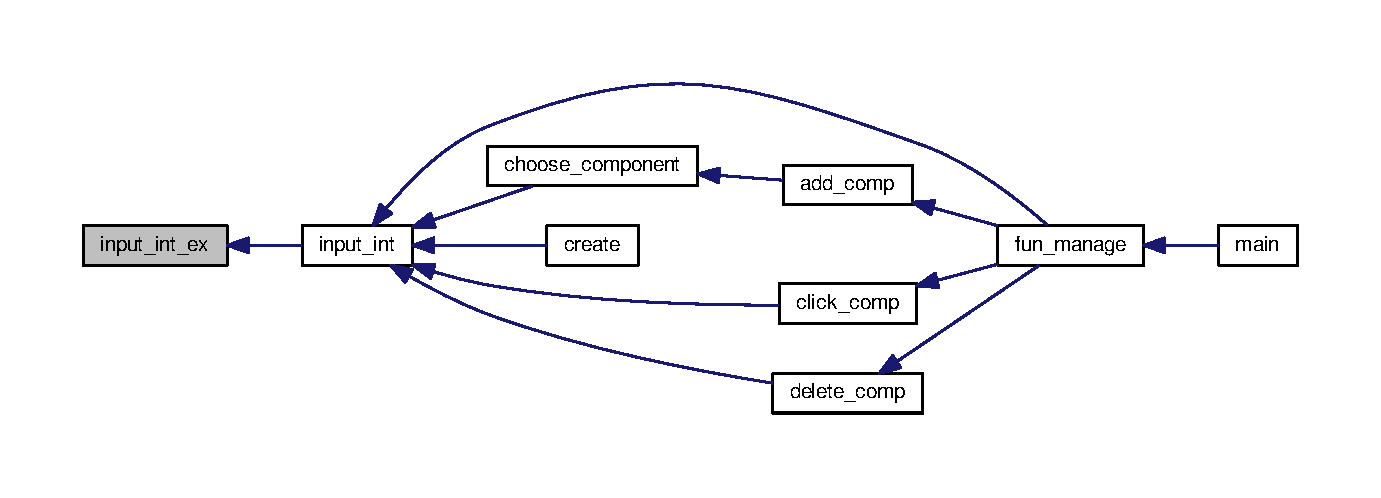
\includegraphics[width=350pt]{operating__sys_8h_a1fb6c8e60497cc915d5bb21a1d2a3e8e_icgraph}
\end{center}
\end{figure}



\hypertarget{window_8cpp}{}\section{Dokumentacja pliku window.\+cpp}
\label{window_8cpp}\index{window.\+cpp@{window.\+cpp}}
{\ttfamily \#include $<$iostream$>$}\\*
{\ttfamily \#include $<$vector$>$}\\*
{\ttfamily \#include \char`\"{}window.\+h\char`\"{}}\\*
Wykres zależności załączania dla window.\+cpp\+:\nopagebreak
\begin{figure}[H]
\begin{center}
\leavevmode
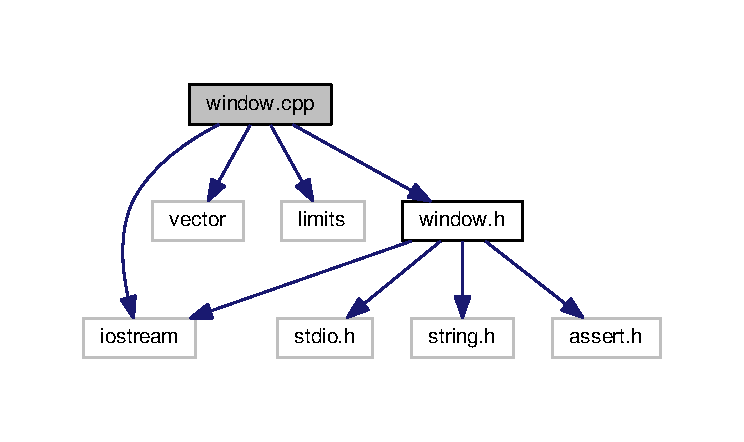
\includegraphics[width=336pt]{window_8cpp__incl}
\end{center}
\end{figure}

\hypertarget{window_8h}{}\section{Dokumentacja pliku window.\+h}
\label{window_8h}\index{window.\+h@{window.\+h}}
{\ttfamily \#include $<$iostream$>$}\\*
{\ttfamily \#include $<$stdio.\+h$>$}\\*
{\ttfamily \#include $<$string.\+h$>$}\\*
{\ttfamily \#include $<$assert.\+h$>$}\\*
Wykres zależności załączania dla window.\+h\+:\nopagebreak
\begin{figure}[H]
\begin{center}
\leavevmode
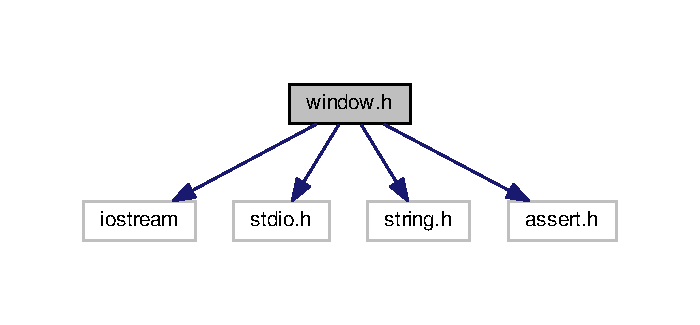
\includegraphics[width=336pt]{window_8h__incl}
\end{center}
\end{figure}
Ten wykres pokazuje, które pliki bezpośrednio lub pośrednio załączają ten plik\+:\nopagebreak
\begin{figure}[H]
\begin{center}
\leavevmode
\includegraphics[width=336pt]{window_8h__dep__incl}
\end{center}
\end{figure}
\subsection*{Komponenty}
\begin{DoxyCompactItemize}
\item 
class \hyperlink{classComponent}{Component}
\item 
class \hyperlink{classText}{Text}
\item 
class \hyperlink{classButton}{Button}
\item 
class \hyperlink{classCheckbox}{Checkbox}
\item 
class \hyperlink{classInput__table}{Input\+\_\+table}
\item 
class \hyperlink{classList}{List}
\end{DoxyCompactItemize}

%--- End generated contents ---

% Index
\backmatter
\newpage
\phantomsection
\clearemptydoublepage
\addcontentsline{toc}{chapter}{Indeks}
\printindex

\end{document}
